\chapter{Results \& Discussion}
\label{Chapter4}
\lhead{Chapter 4. \emph{Results \& Discussion}}
We hereby present the results of the computational investigations of CSH performed throughout this work. The results are organised into the following main sections: \textbf{i}) Optimal bulk parameters and Density of States (DOS) calculations, \textbf{ii}) MLFF training, refinement and validation, \textbf{iii}) Themodynamic properties of CSH, and \textbf{iv}) Transferability of MLFFs and thermal expansion coefficient of CSH. 
 
\section{Optimal Bulk Parameters and Density of States (DOS) calculations}

\subsection{Cut-off Energy}
The cut-off energy is essential in VASP calculations as it determines the maximum kinetic energy of the plane-wave basis set. As such, it ensures the completeness of this basis set and the accurate description of the electroic structure of the system.  The cut-off energy convergence test herein presented was conducted using the PBEsol functional. As shown in Figure \ref{cutoff-energy}, an optimal $E_{\text{cut}}$ is achieved at 800 eV, where the convergence criteria of 1 meV/atom is satisfied. The notably high cut-off energy can be atributed to the presence of heavy elements in the CSH structure, such as Calcium (Ca) and Silicon (Si), which require a high cut-off energy values\supercite{zotero-item-698}. All the subsequent VASP calculations were performed using this cut-off energy value.
\begin{figure}[H]
    \centering
    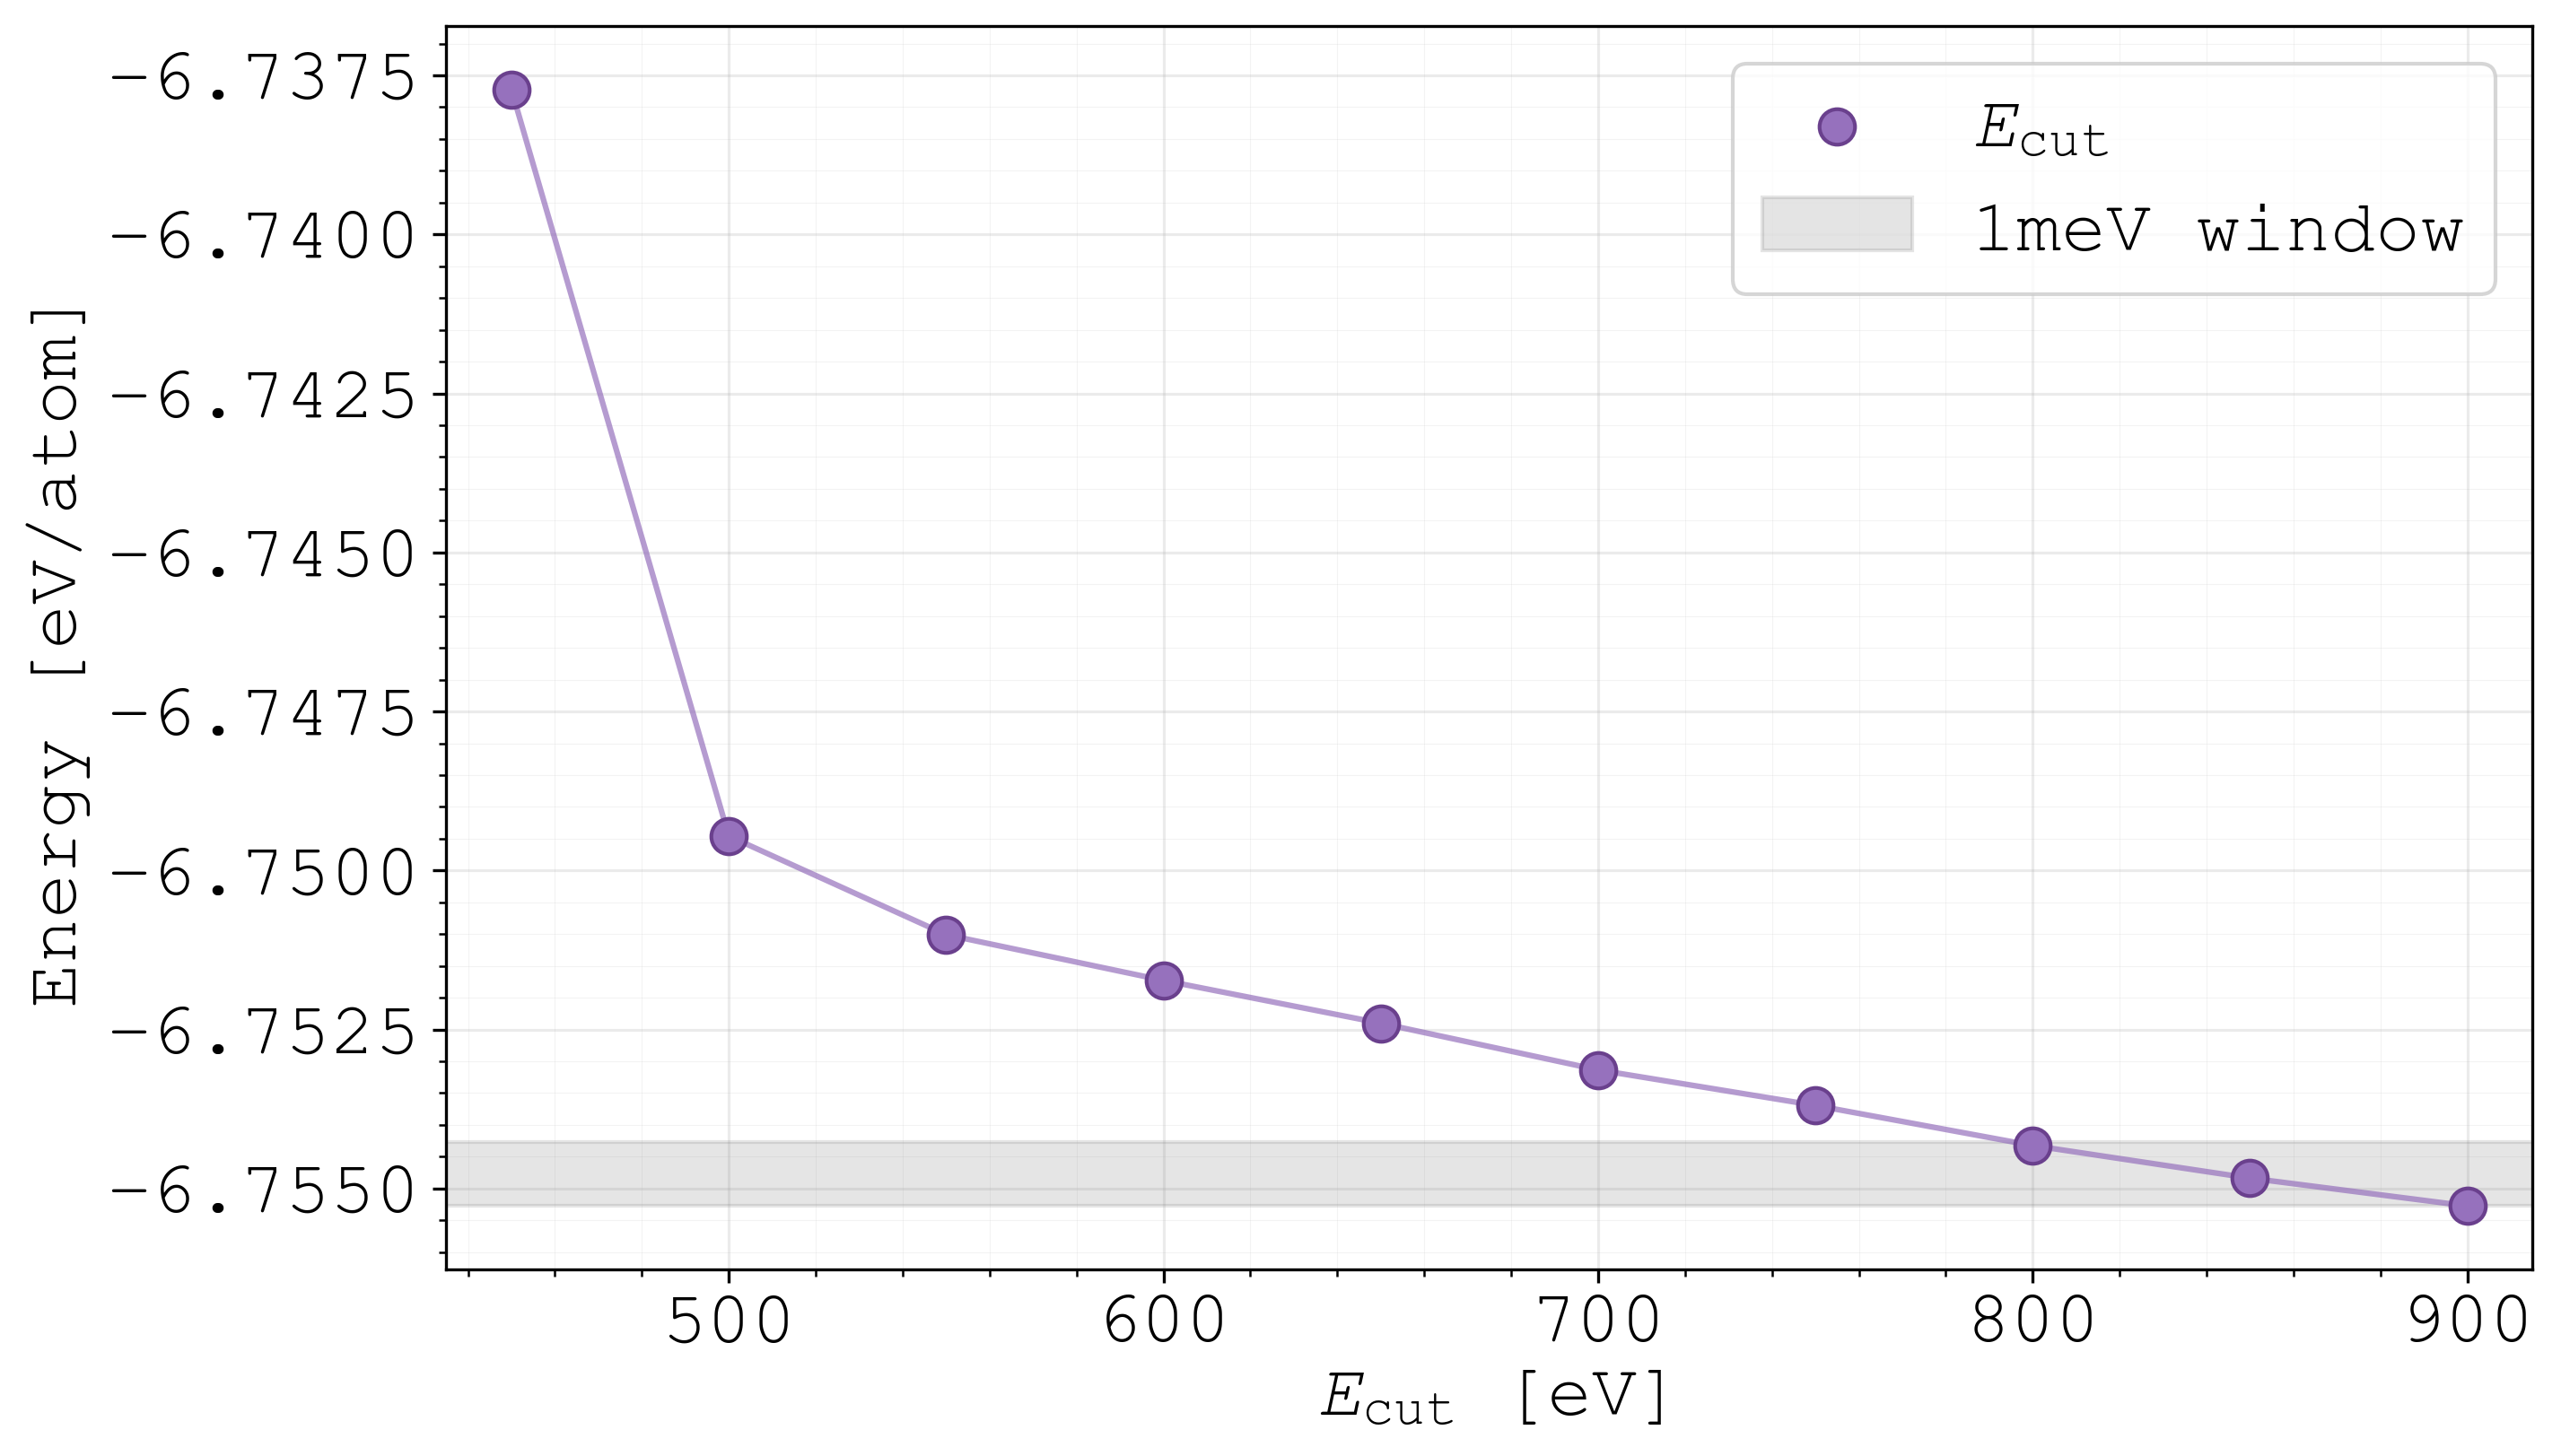
\includegraphics[width=0.8\textwidth]{cutoff-vasp.png}
    \caption{
    Cut-off energy convergence test performed in VASP employing the PBEsol functional for $300 \leq E_{\text{cut}} \leq 900$ eV. The $\Delta E = 1$meV/atom convergence criteria is achieved at $E_{\text {cut}} = 800$ eV}
    \label{cutoff-energy}
\end{figure}

\subsection{k-point convergence}
 Two k-point convergence tests were performed, one previous to the initial relaxation of the CSH structure using DFTB+ (see Figure \ref{dftb-kpoints}), and the other one (see Figure \ref{kpoints-vasp}) before running the full relaxation in VASP. A ($1\times 1\times 1$) $\Gamma$-centered k-point mesh was adopted for both cases as it satisfies the convergence criteria of $\Delta E= 1$ meV/atom. 
\begin{figure}[H]
    \centering
    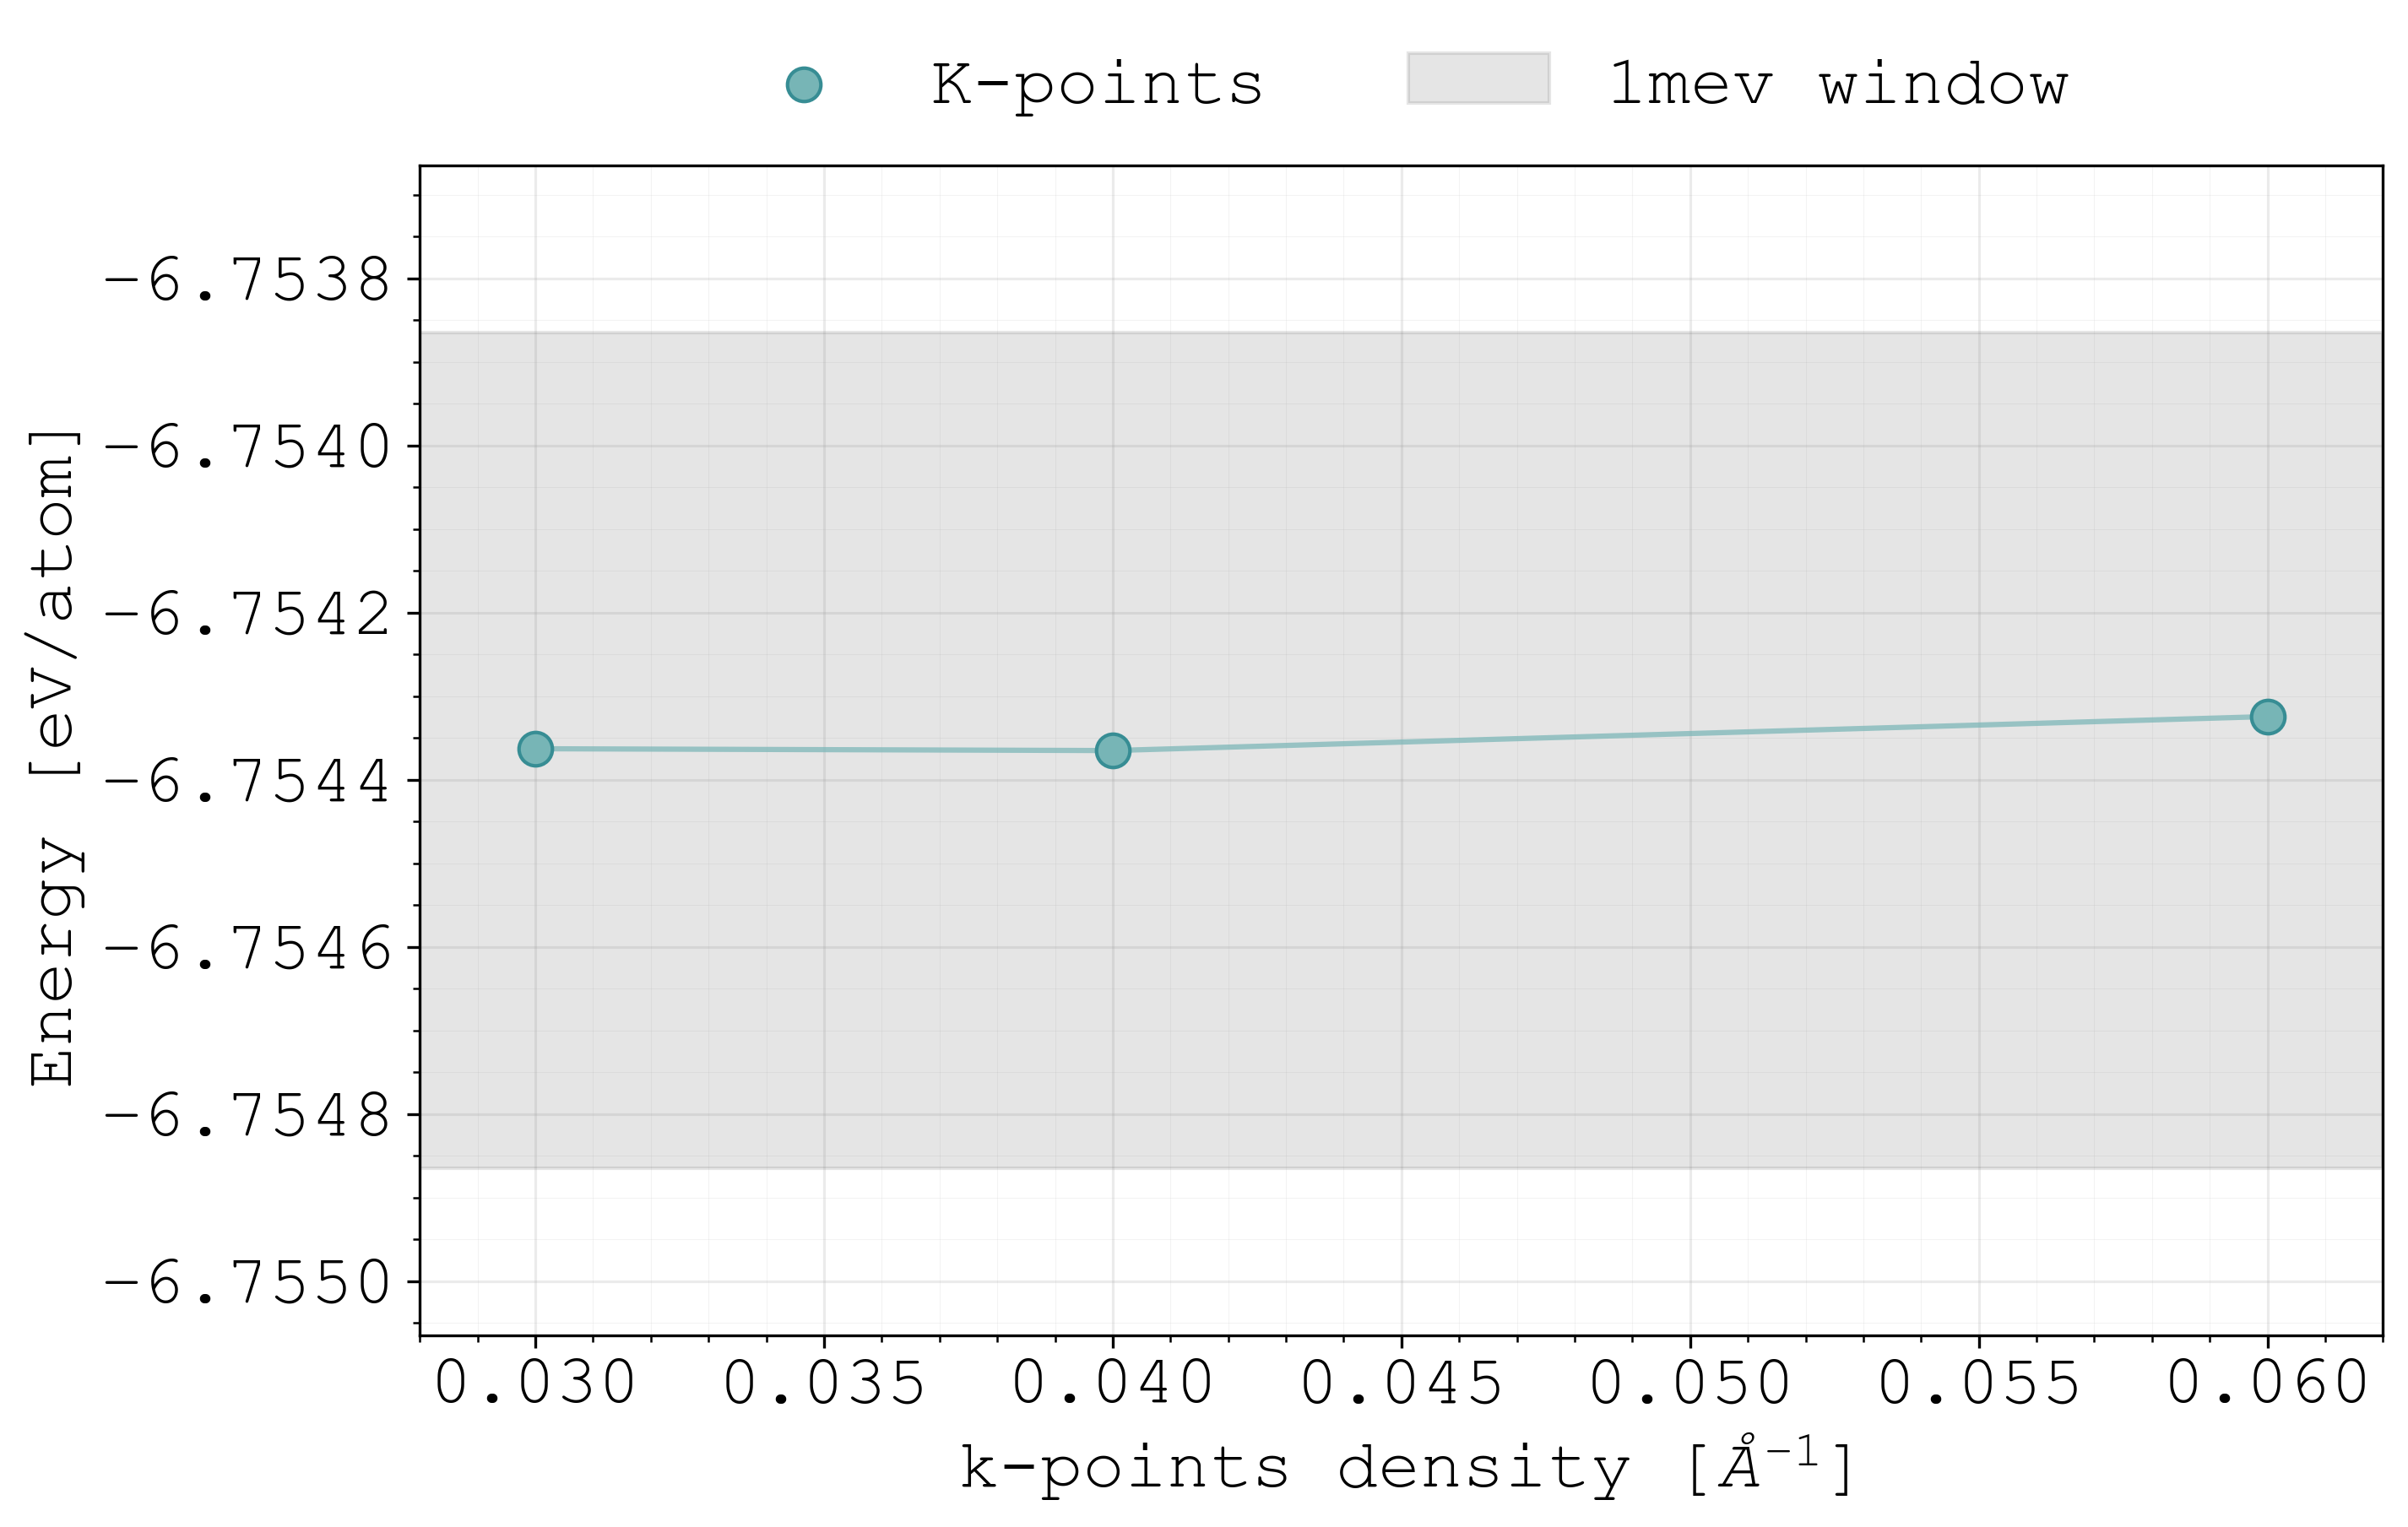
\includegraphics[width=0.8\textwidth]{dftb-kpoints.png}
    \caption{k-point convergence test performed in DFTB+ using the GFN1-xTB method for $0.03 \leq \Delta k \leq 0.06$. The 
    $\Delta E = 1$meV/atom convergence criteria is achieved at $\Delta k = 0.06 \,\text{\AA}^{-1}$ corresponding to a $1\times 1\times 1$ k-point grid. 
    }
    \label{dftb-kpoints}
\end{figure}

\begin{figure}[H]
    \centering
    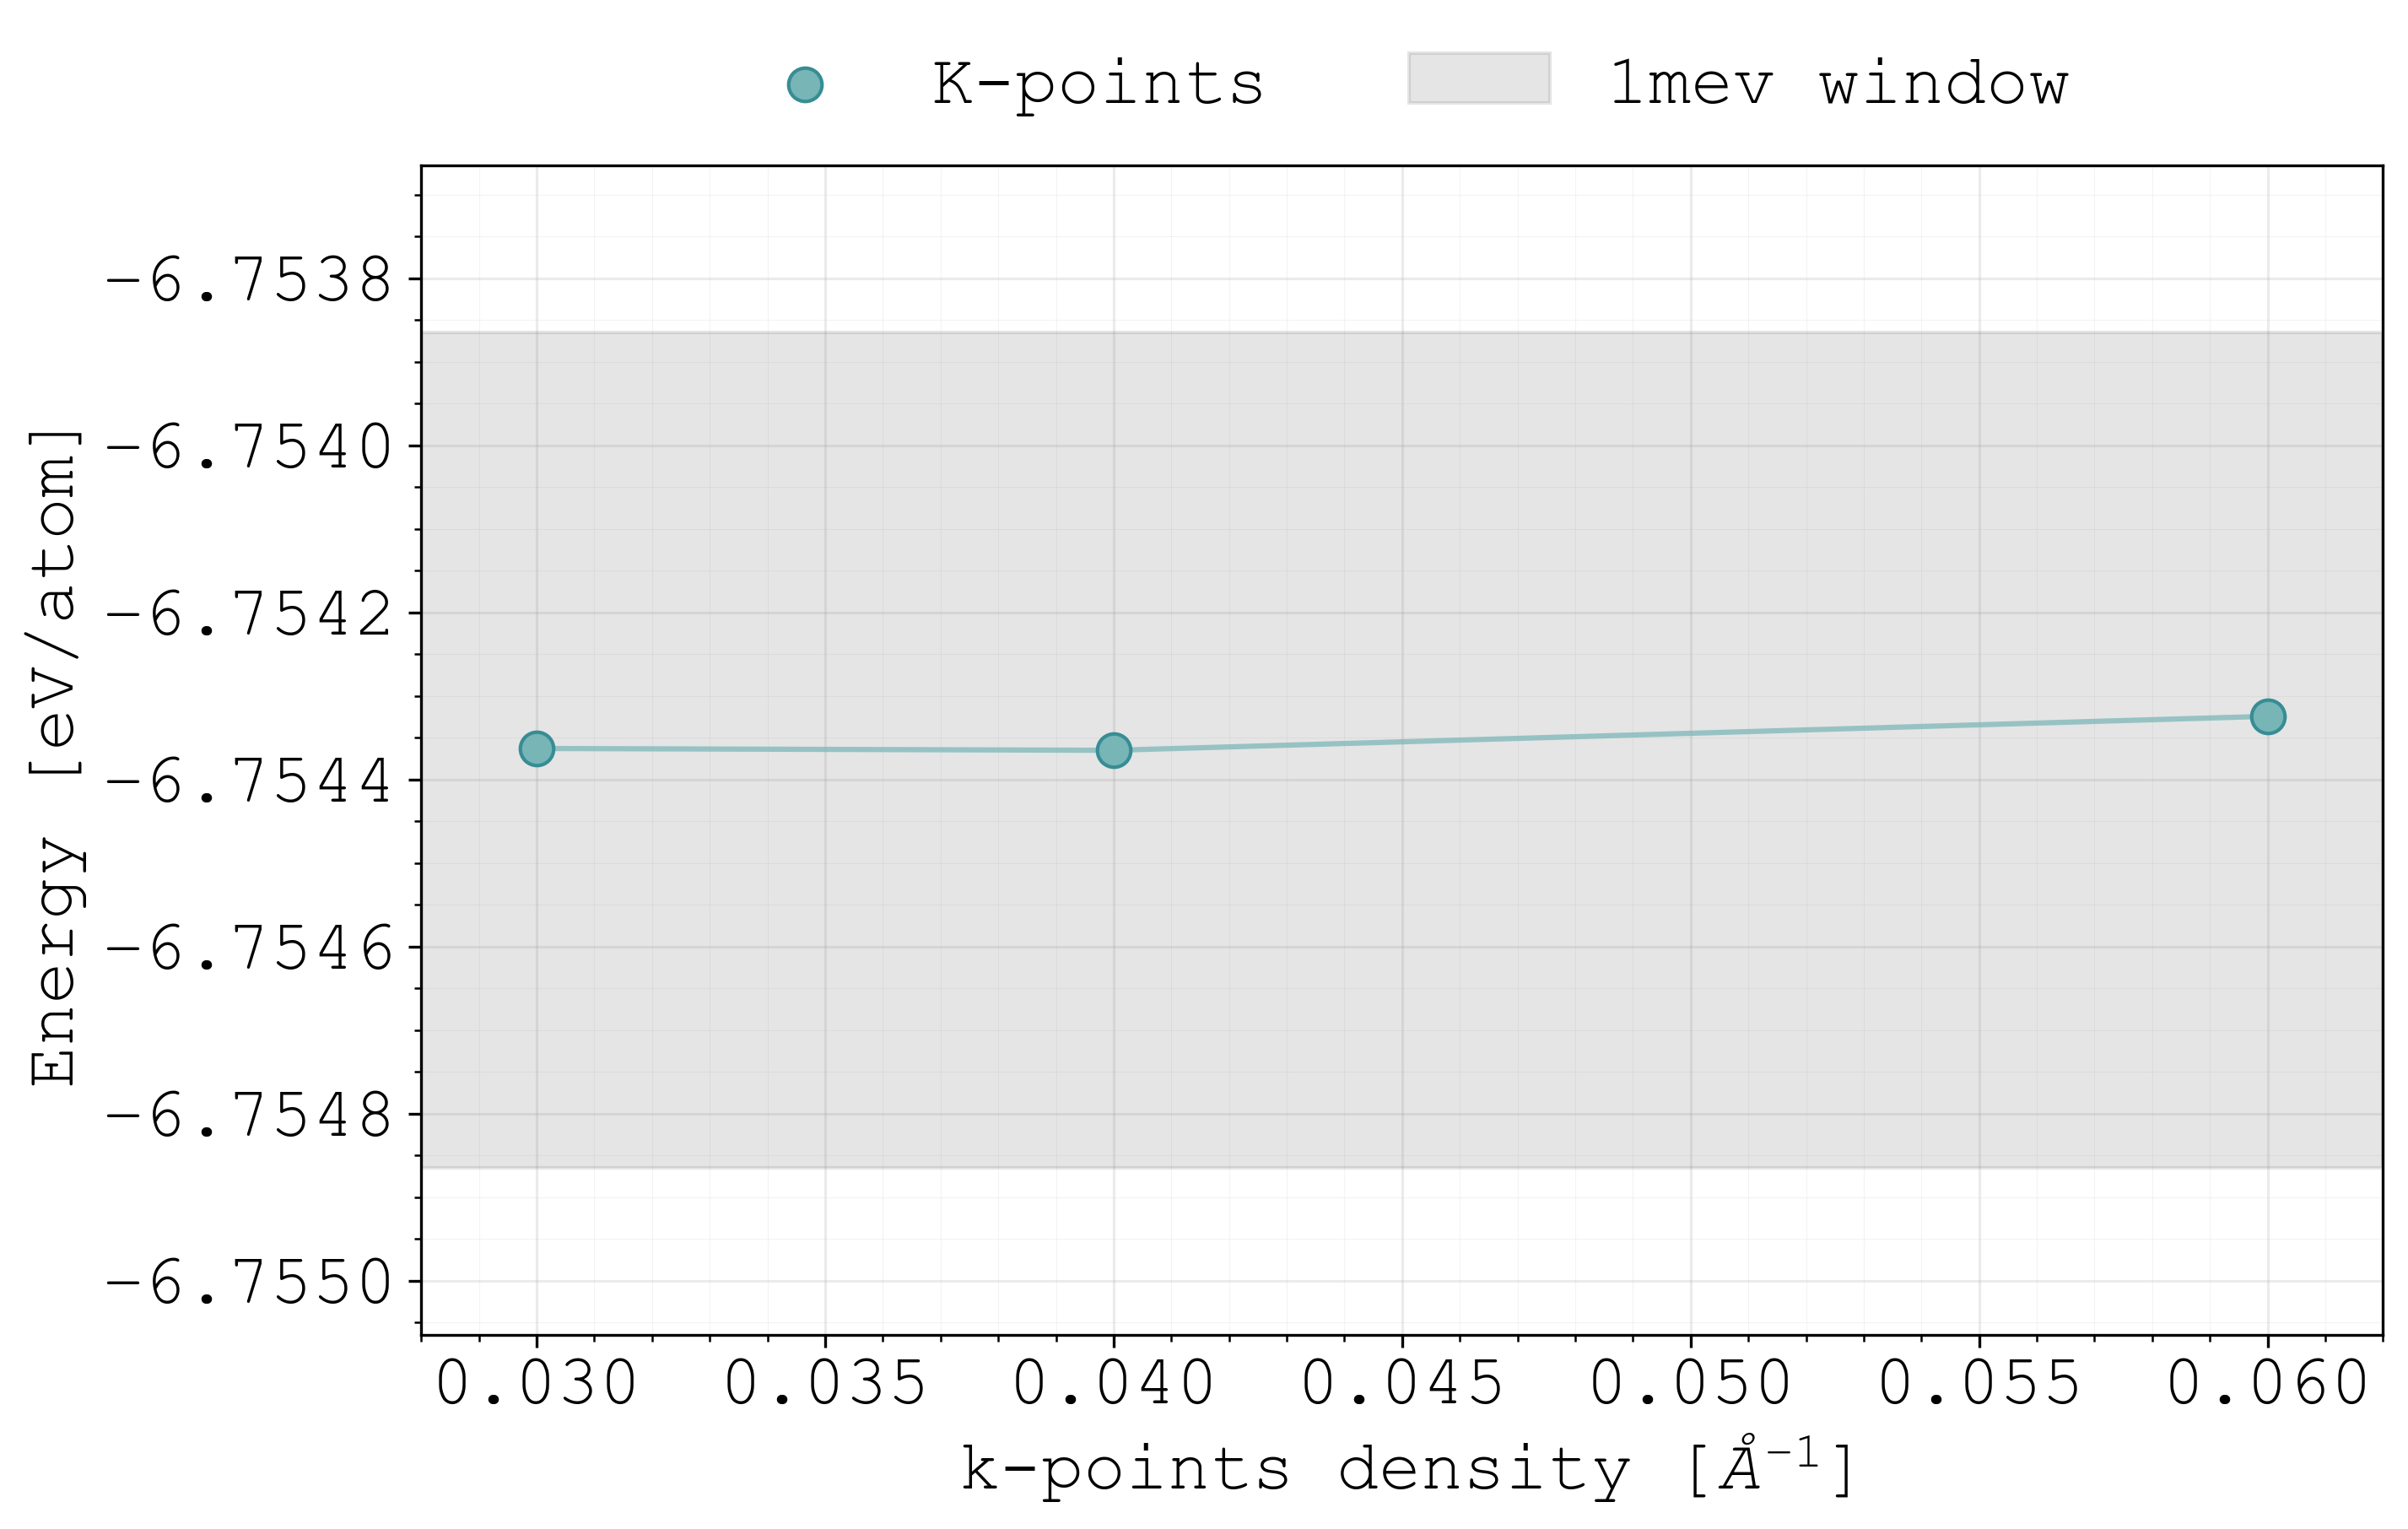
\includegraphics[width=0.8\textwidth]{kpoints-vasp.png}
    \caption{k-point convergence test performed in VASP using the PBEsol functional for $0.03 \leq \Delta k \leq 0.06$. The $\Delta E = 1$meV/atom convergence criteria is achieved at $\Delta k = 0.06 \,\text{\AA}^{-1}$ corresponding to a $1\times 1\times 1$ k-point grid, in agreement with the DFTB+ results.
    }
    \label{kpoints-vasp}
\end{figure}
The k-point convergence test was performed for the GFN1-xTB method in DFTB+ and the PBEsol functional in VASP, both yielding consistent results. 

\subsection{Density of States (DOS)}
The Density of States (DOS) was calculated using the PBEsol functional in VASP. The results presented in Figure \ref{dos}. 
\begin{figure}[H]
    \centering
    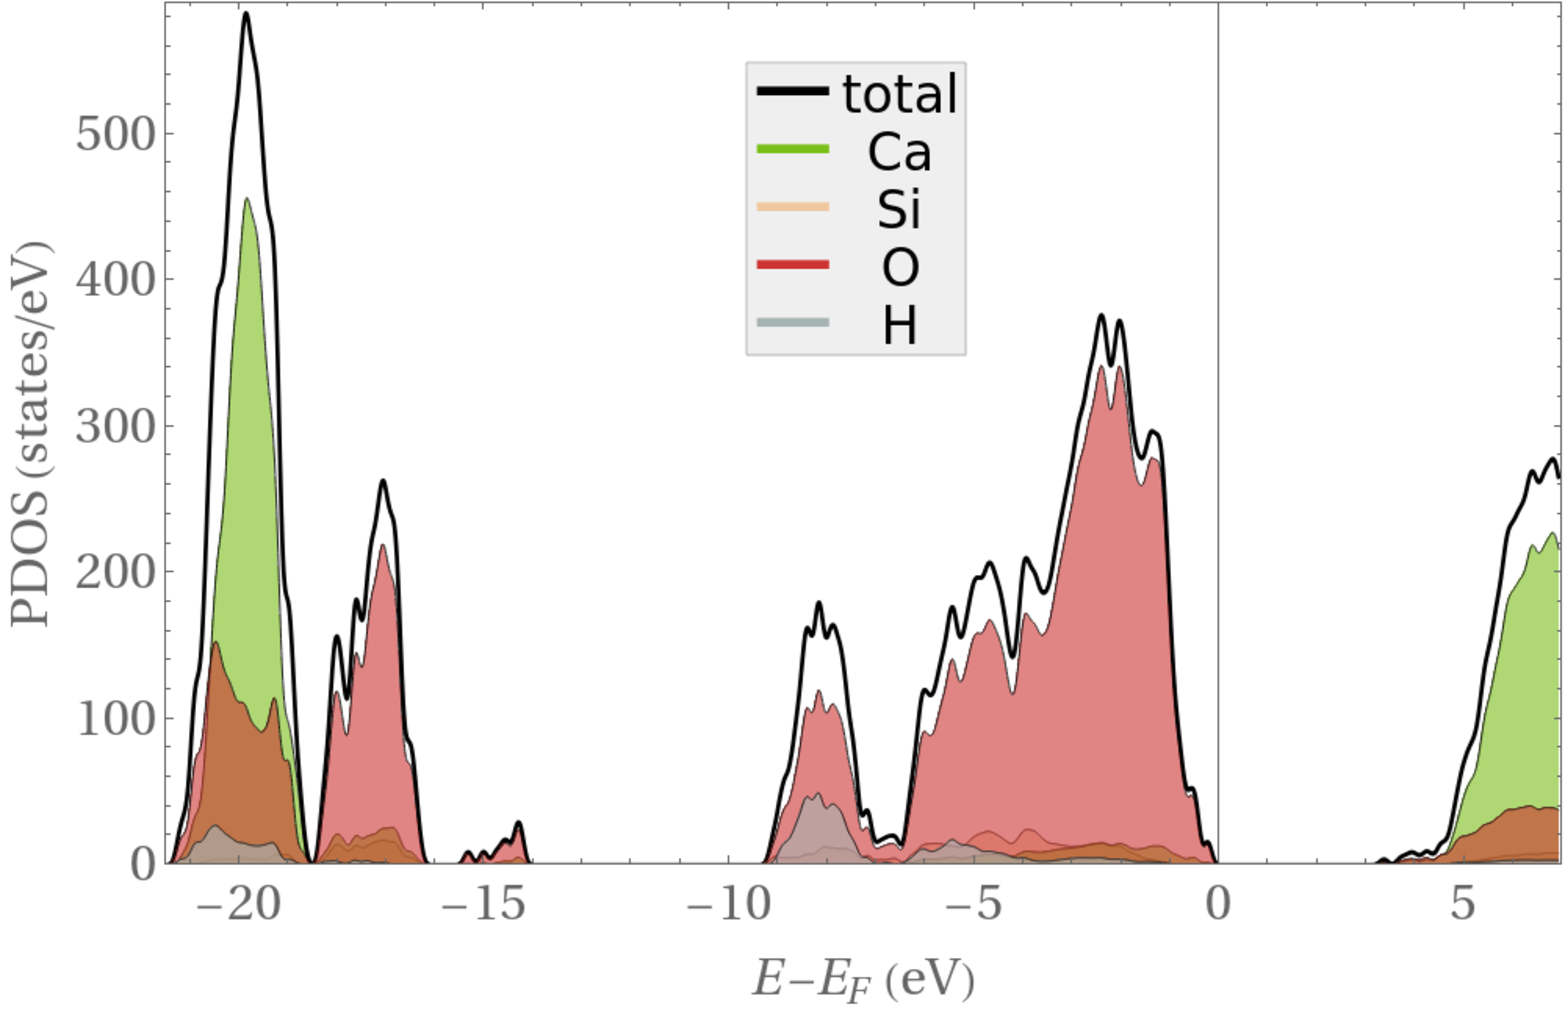
\includegraphics[width=0.7\textwidth]{DOS.pdf}
    \caption{k-point convergence test performed in VASP using the PBEsol functional for $0.03 \leq \Delta k \leq 0.06$. The $\Delta E = 1$meV/atom convergence criteria is achieved at $\Delta k = 0.06 \,\text{\AA}^{-1}$ corresponding to a $1\times 1\times 1$ k-point grid, in agreement with the DFTB+ results.
    }
    \label{dos}
\end{figure}

\section{Machine Learning Force Field (MLFF) Training, Refinement and Validation}
A core aspect of this work is the development of a machine learning force field (MLFF) for CSH. 
\subsection{Training and Refinement}

\begin{figure}[h]
    \centering
    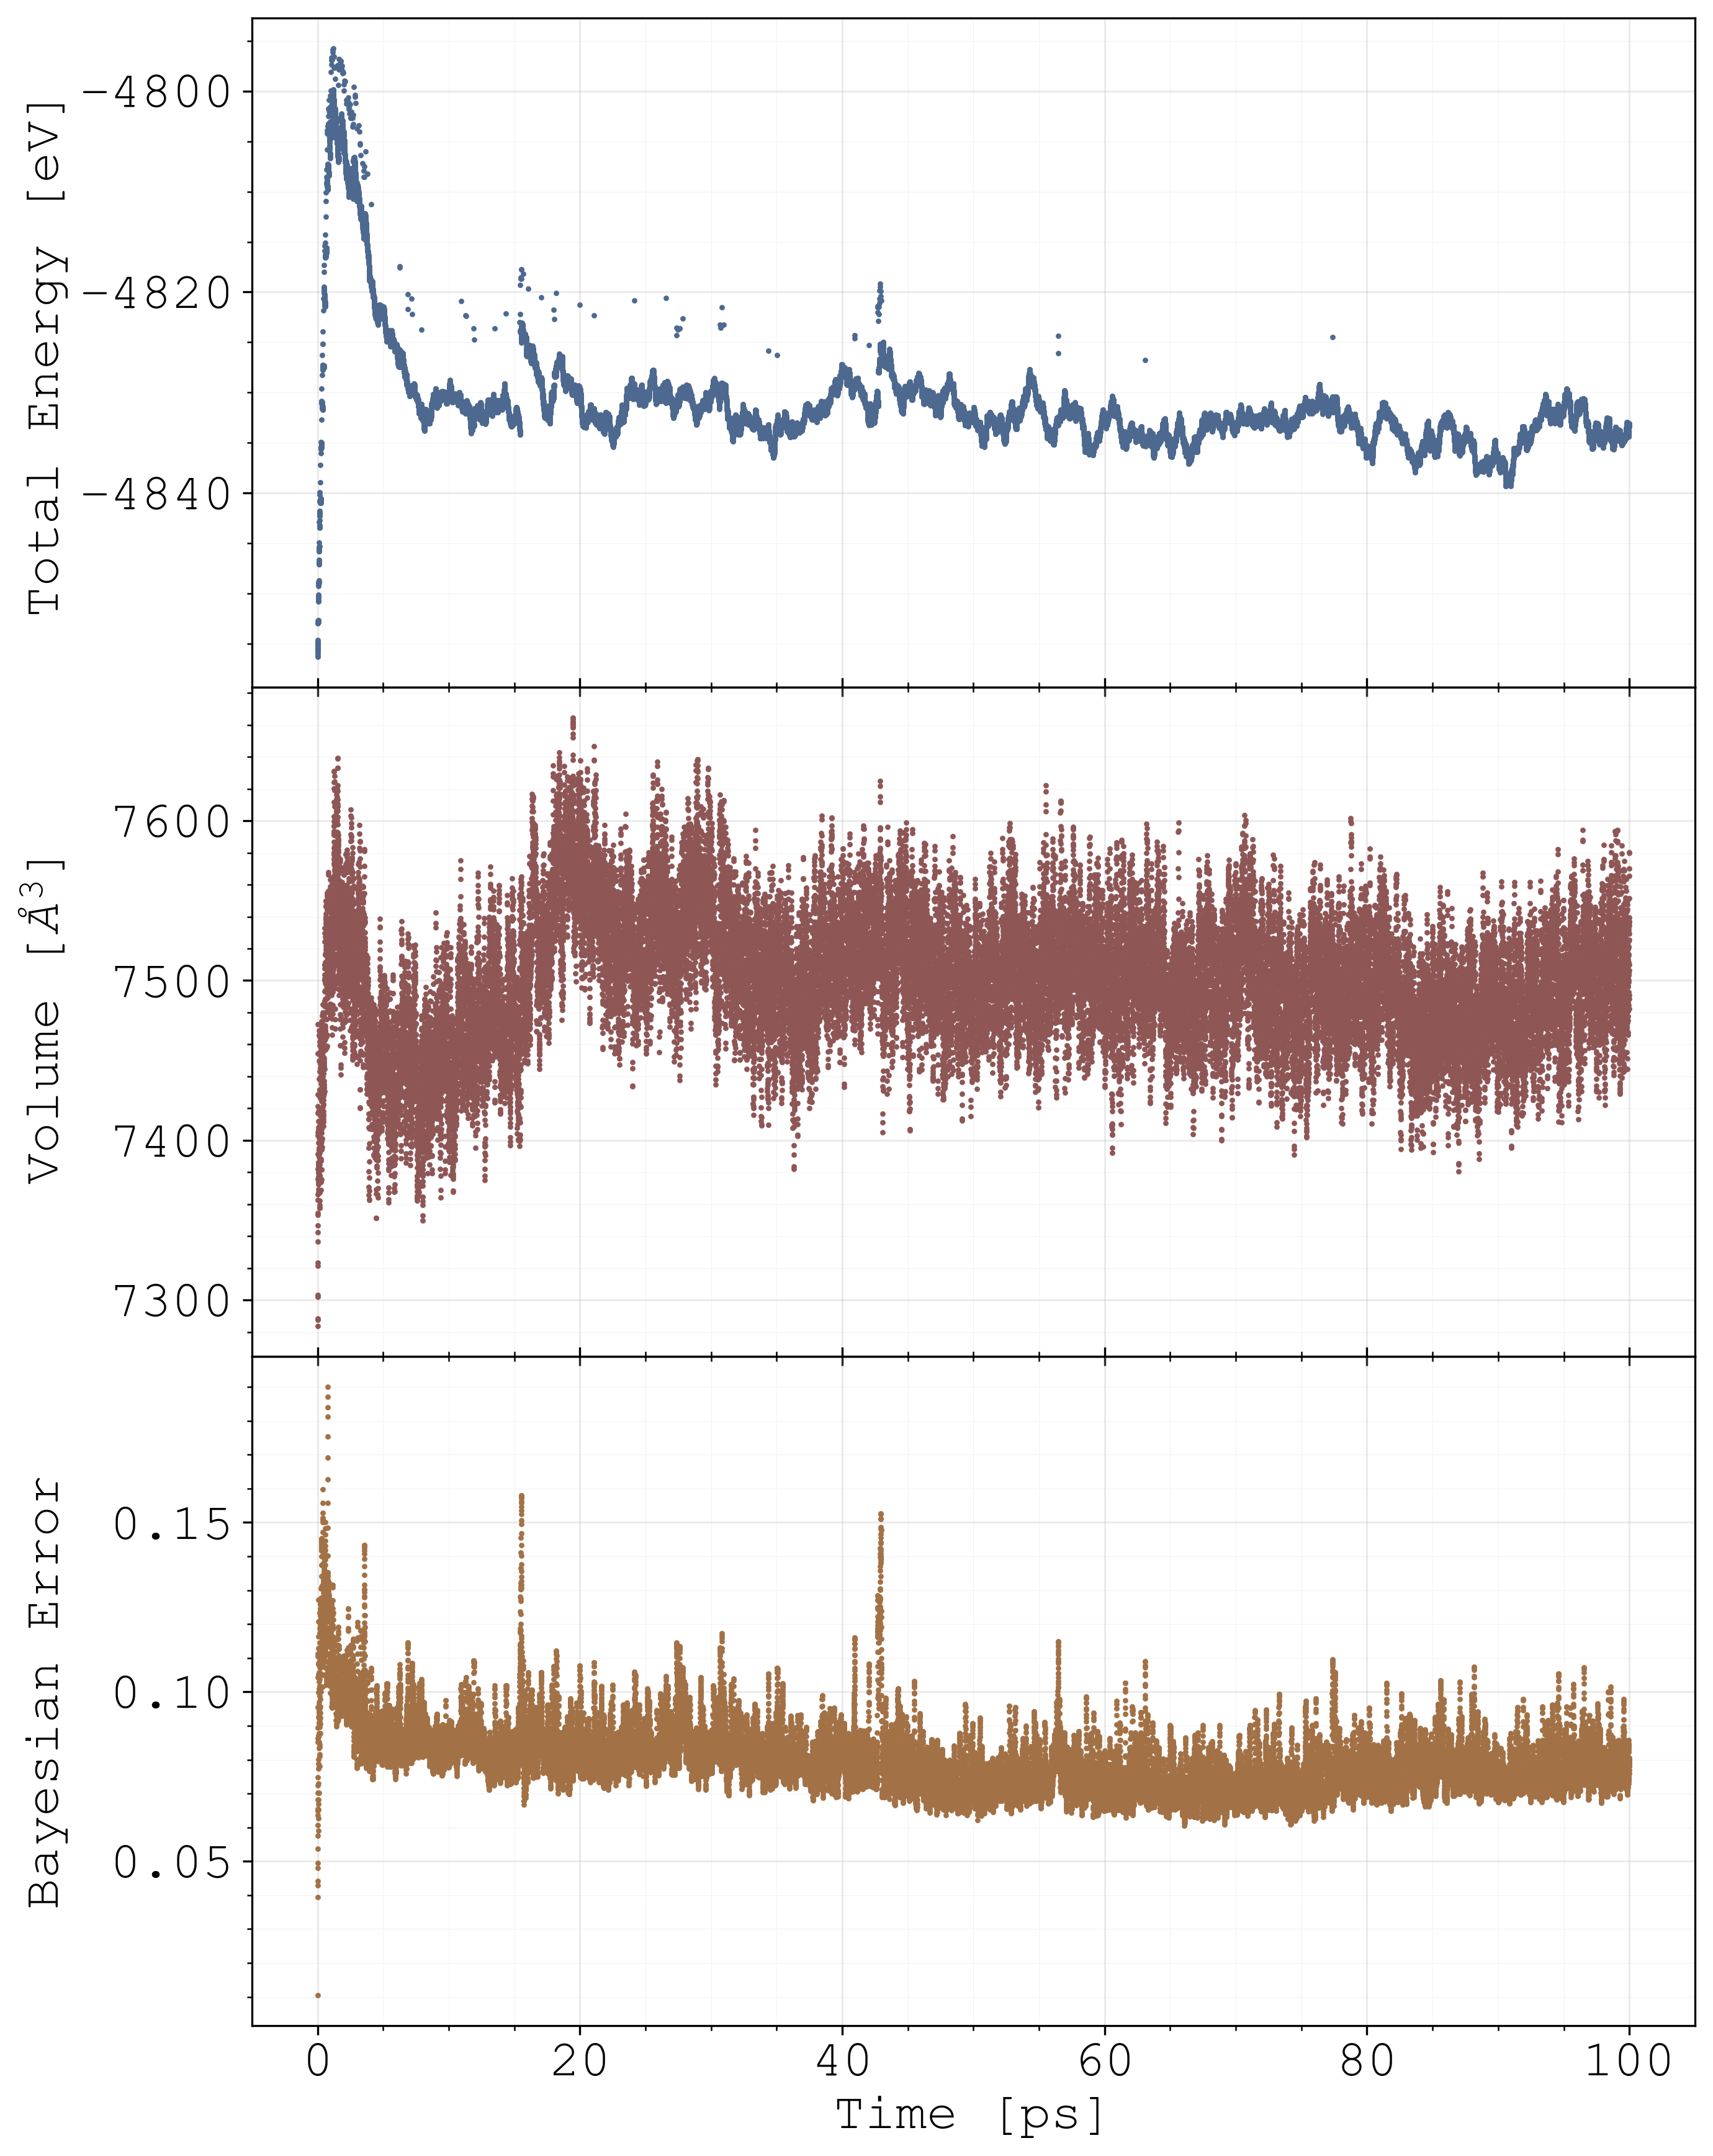
\includegraphics[width=0.8\textwidth]{training-stats.png}
    \caption{
    My label
    }
    \label{training-stats}
\end{figure}


\begin{figure}[h]
    \centering
    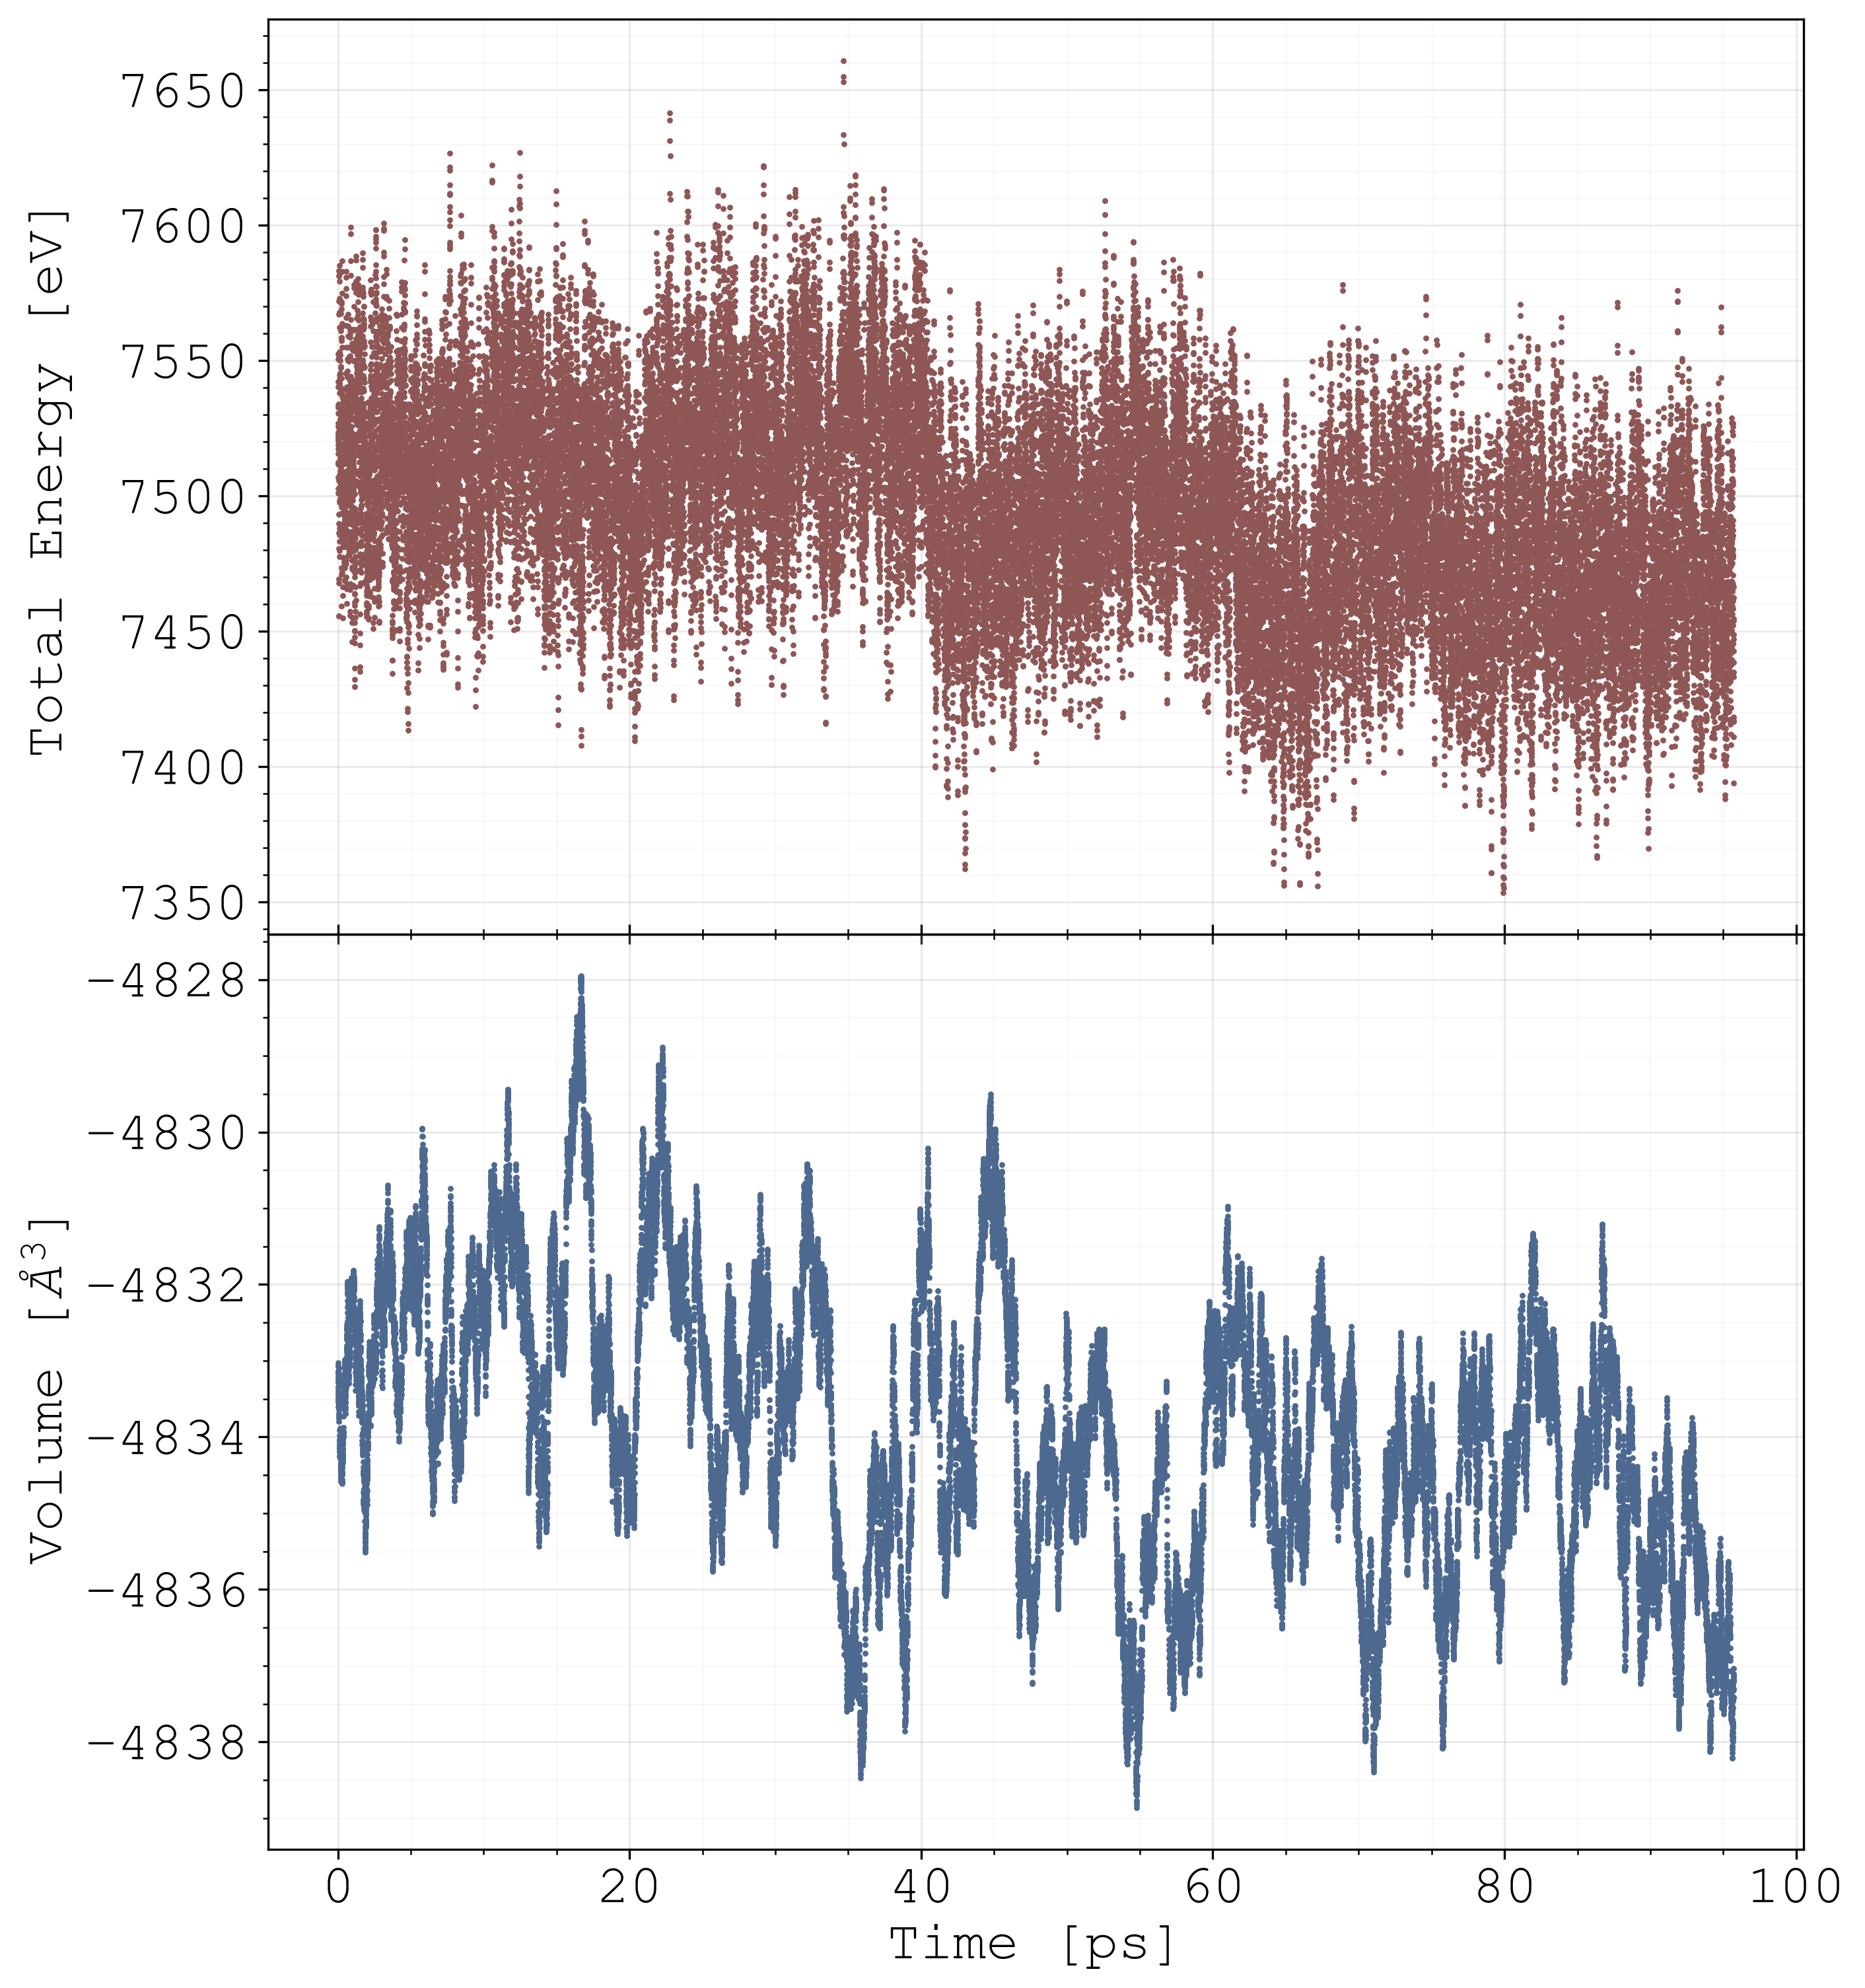
\includegraphics[width=0.8\textwidth]{pred-stats.png}
    \caption{
    My label
    }
    \label{pred-stats}
\end{figure}


\begin{figure}[h]
    \centering
    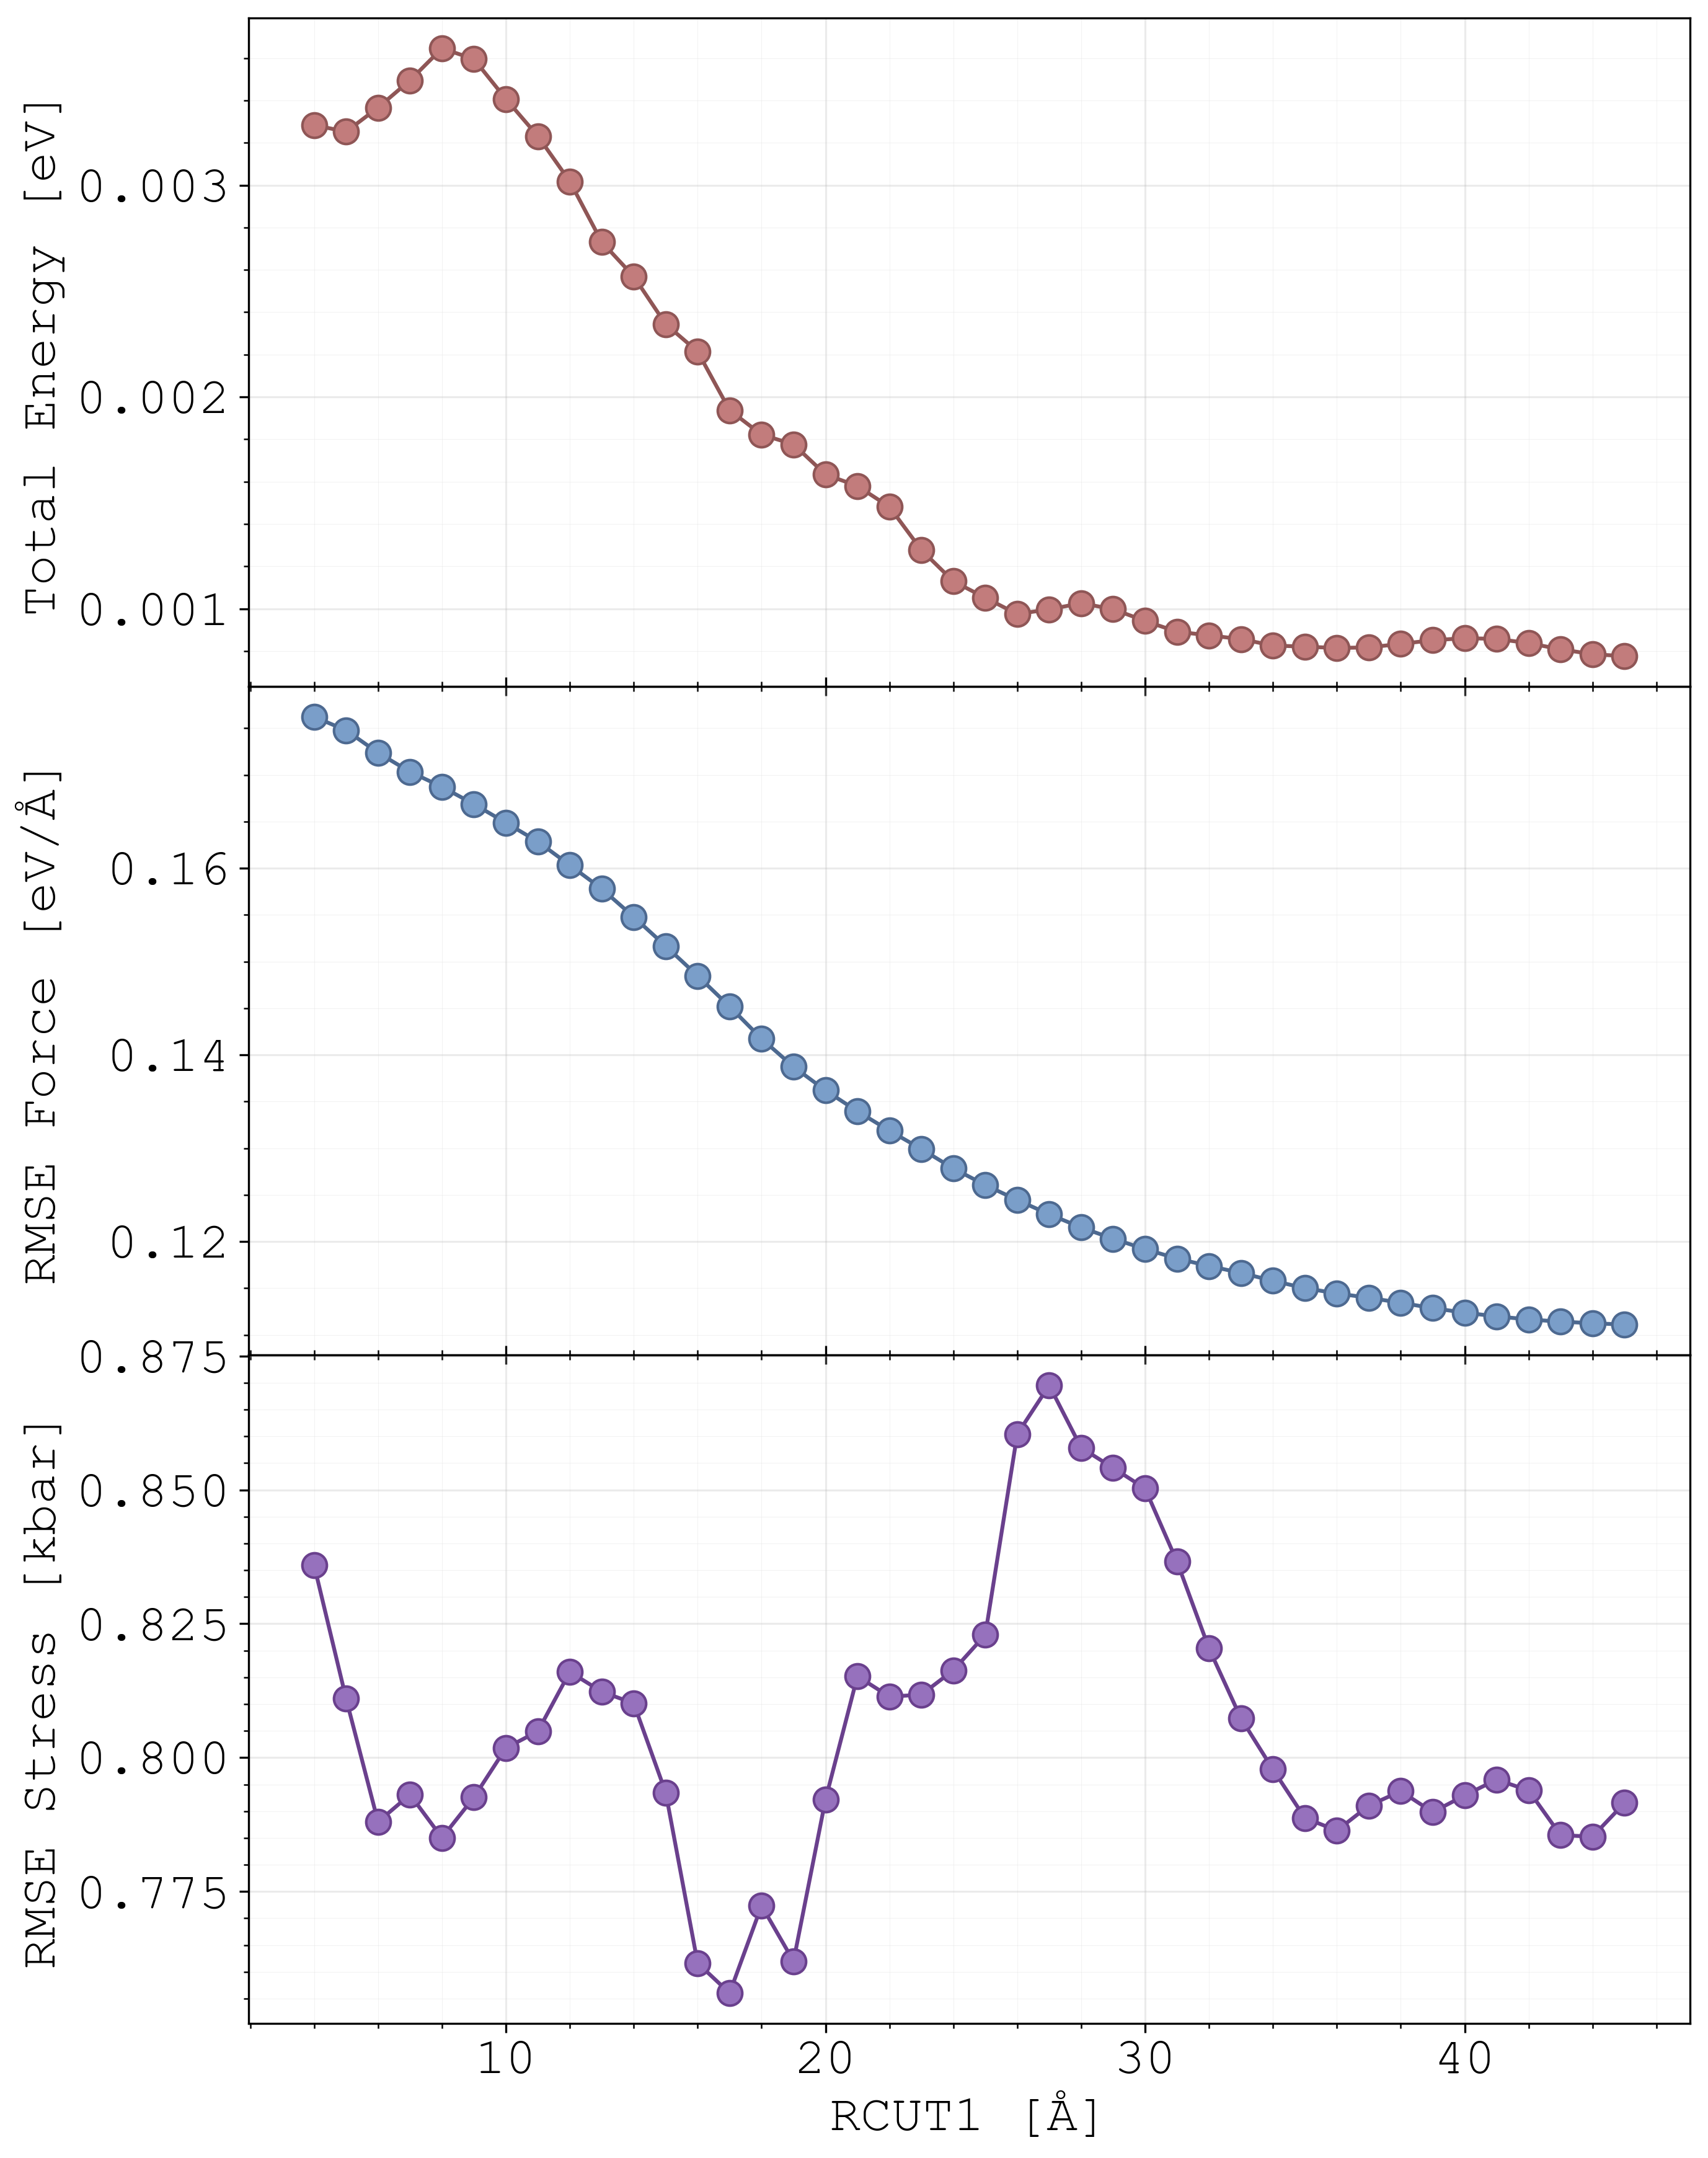
\includegraphics[width=0.8\textwidth]{rcut1.png}
    \caption{
    My label
    }
    \label{rcut1}
\end{figure}

\begin{figure}[h]
    \centering
    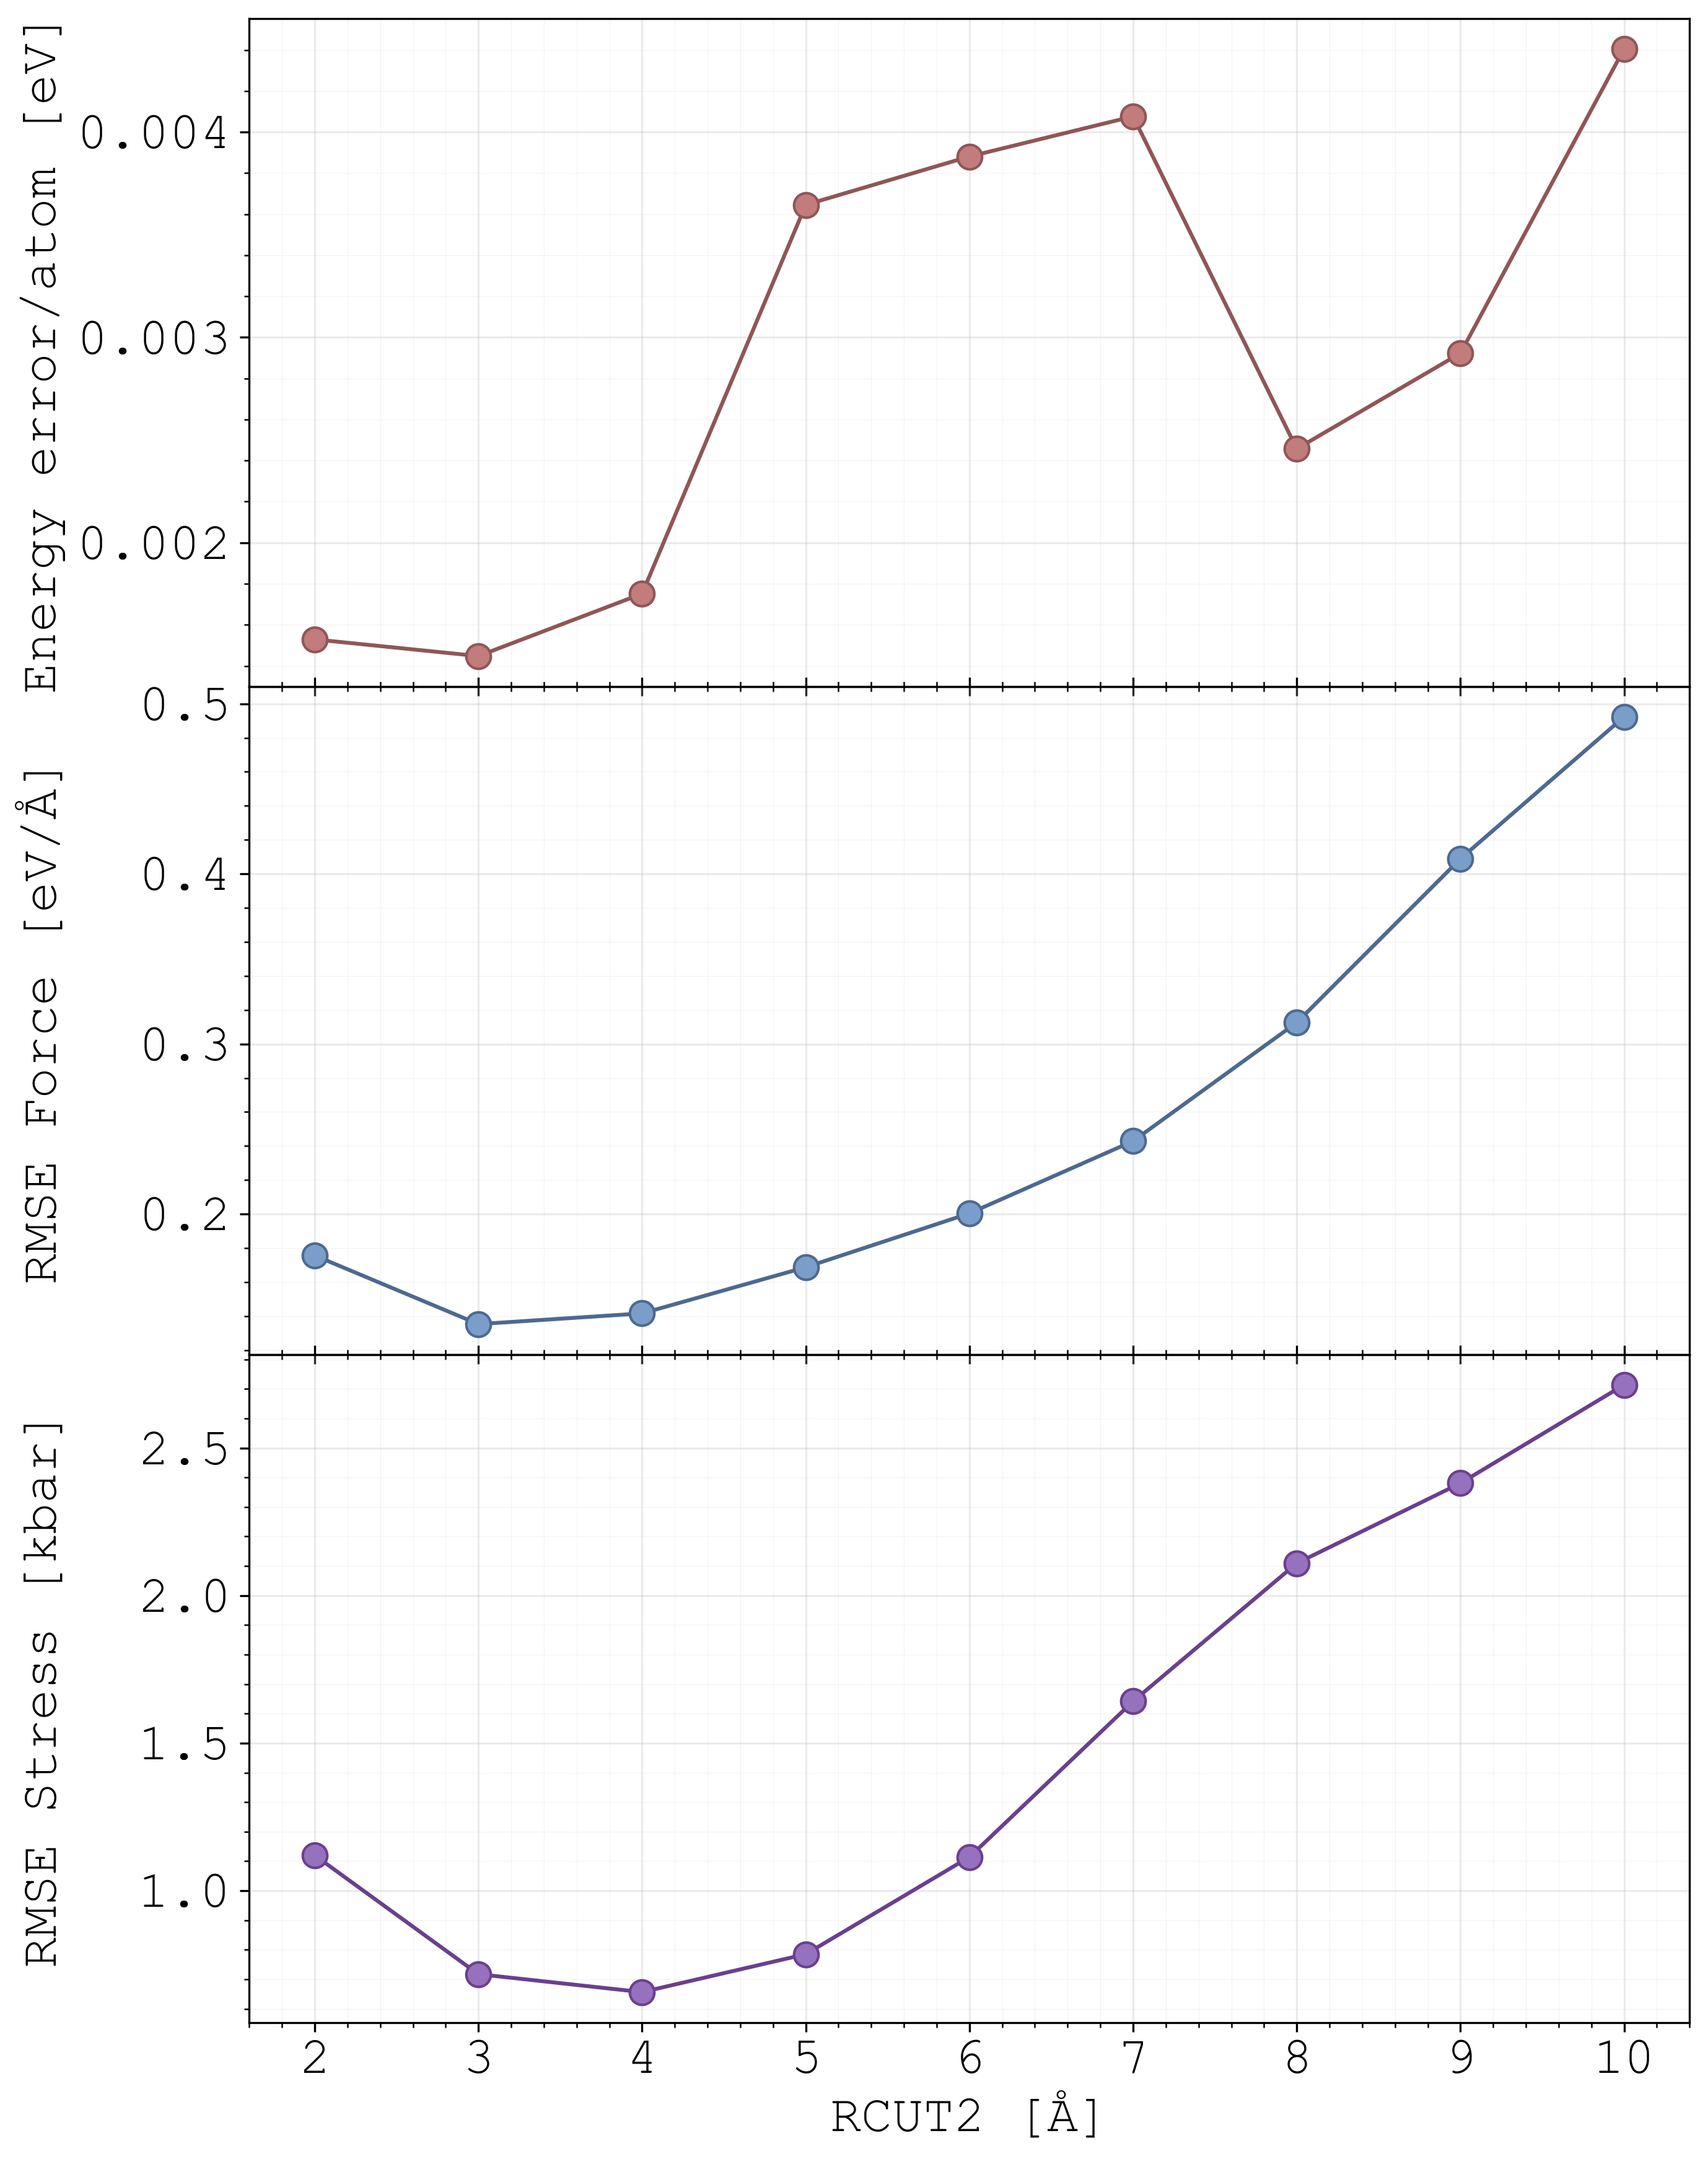
\includegraphics[width=0.8\textwidth]{rcut2.png}
    \caption{
    My label
    }
    \label{rcut2}
\end{figure}

\subsection{Validation}


\section{Thermodynamic Properties of CSH}




\begin{figure}[h]
    \centering
    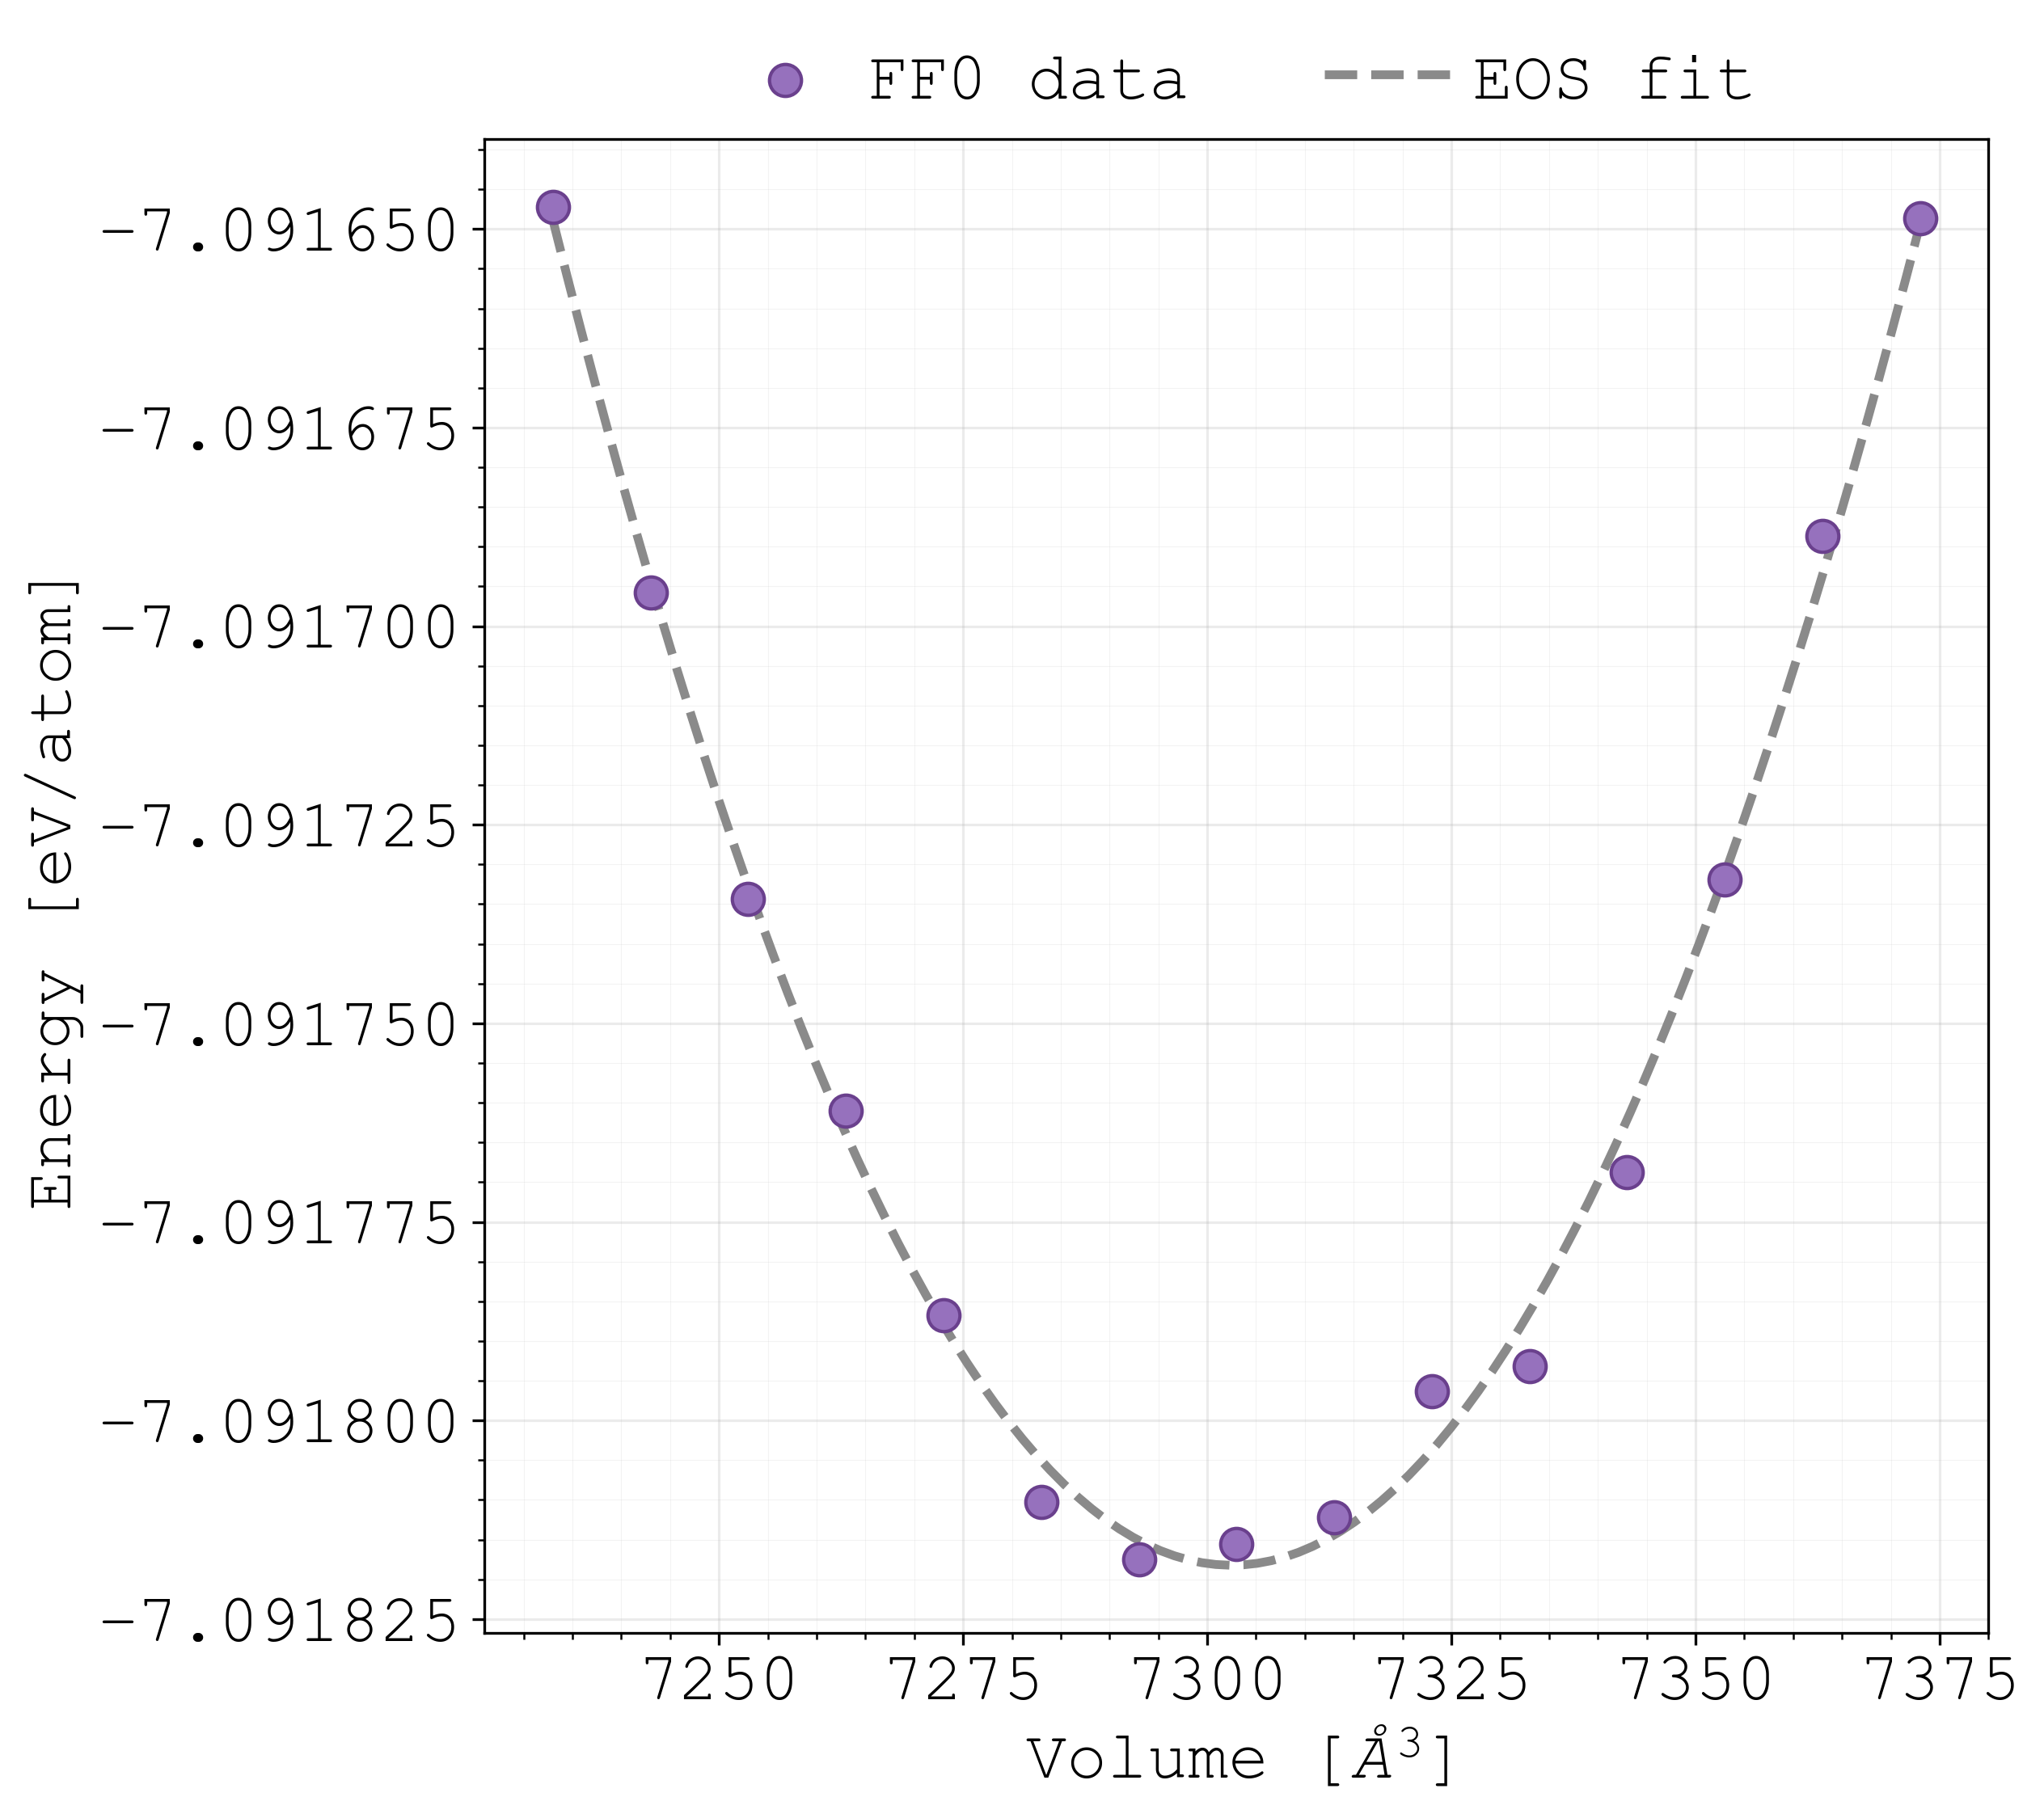
\includegraphics[width=0.7\textwidth]{EOS-FF0.png}
    \caption{Hey}
    \label{fig:eos-ff0}
\end{figure}


\begin{figure}[h]
    \centering
    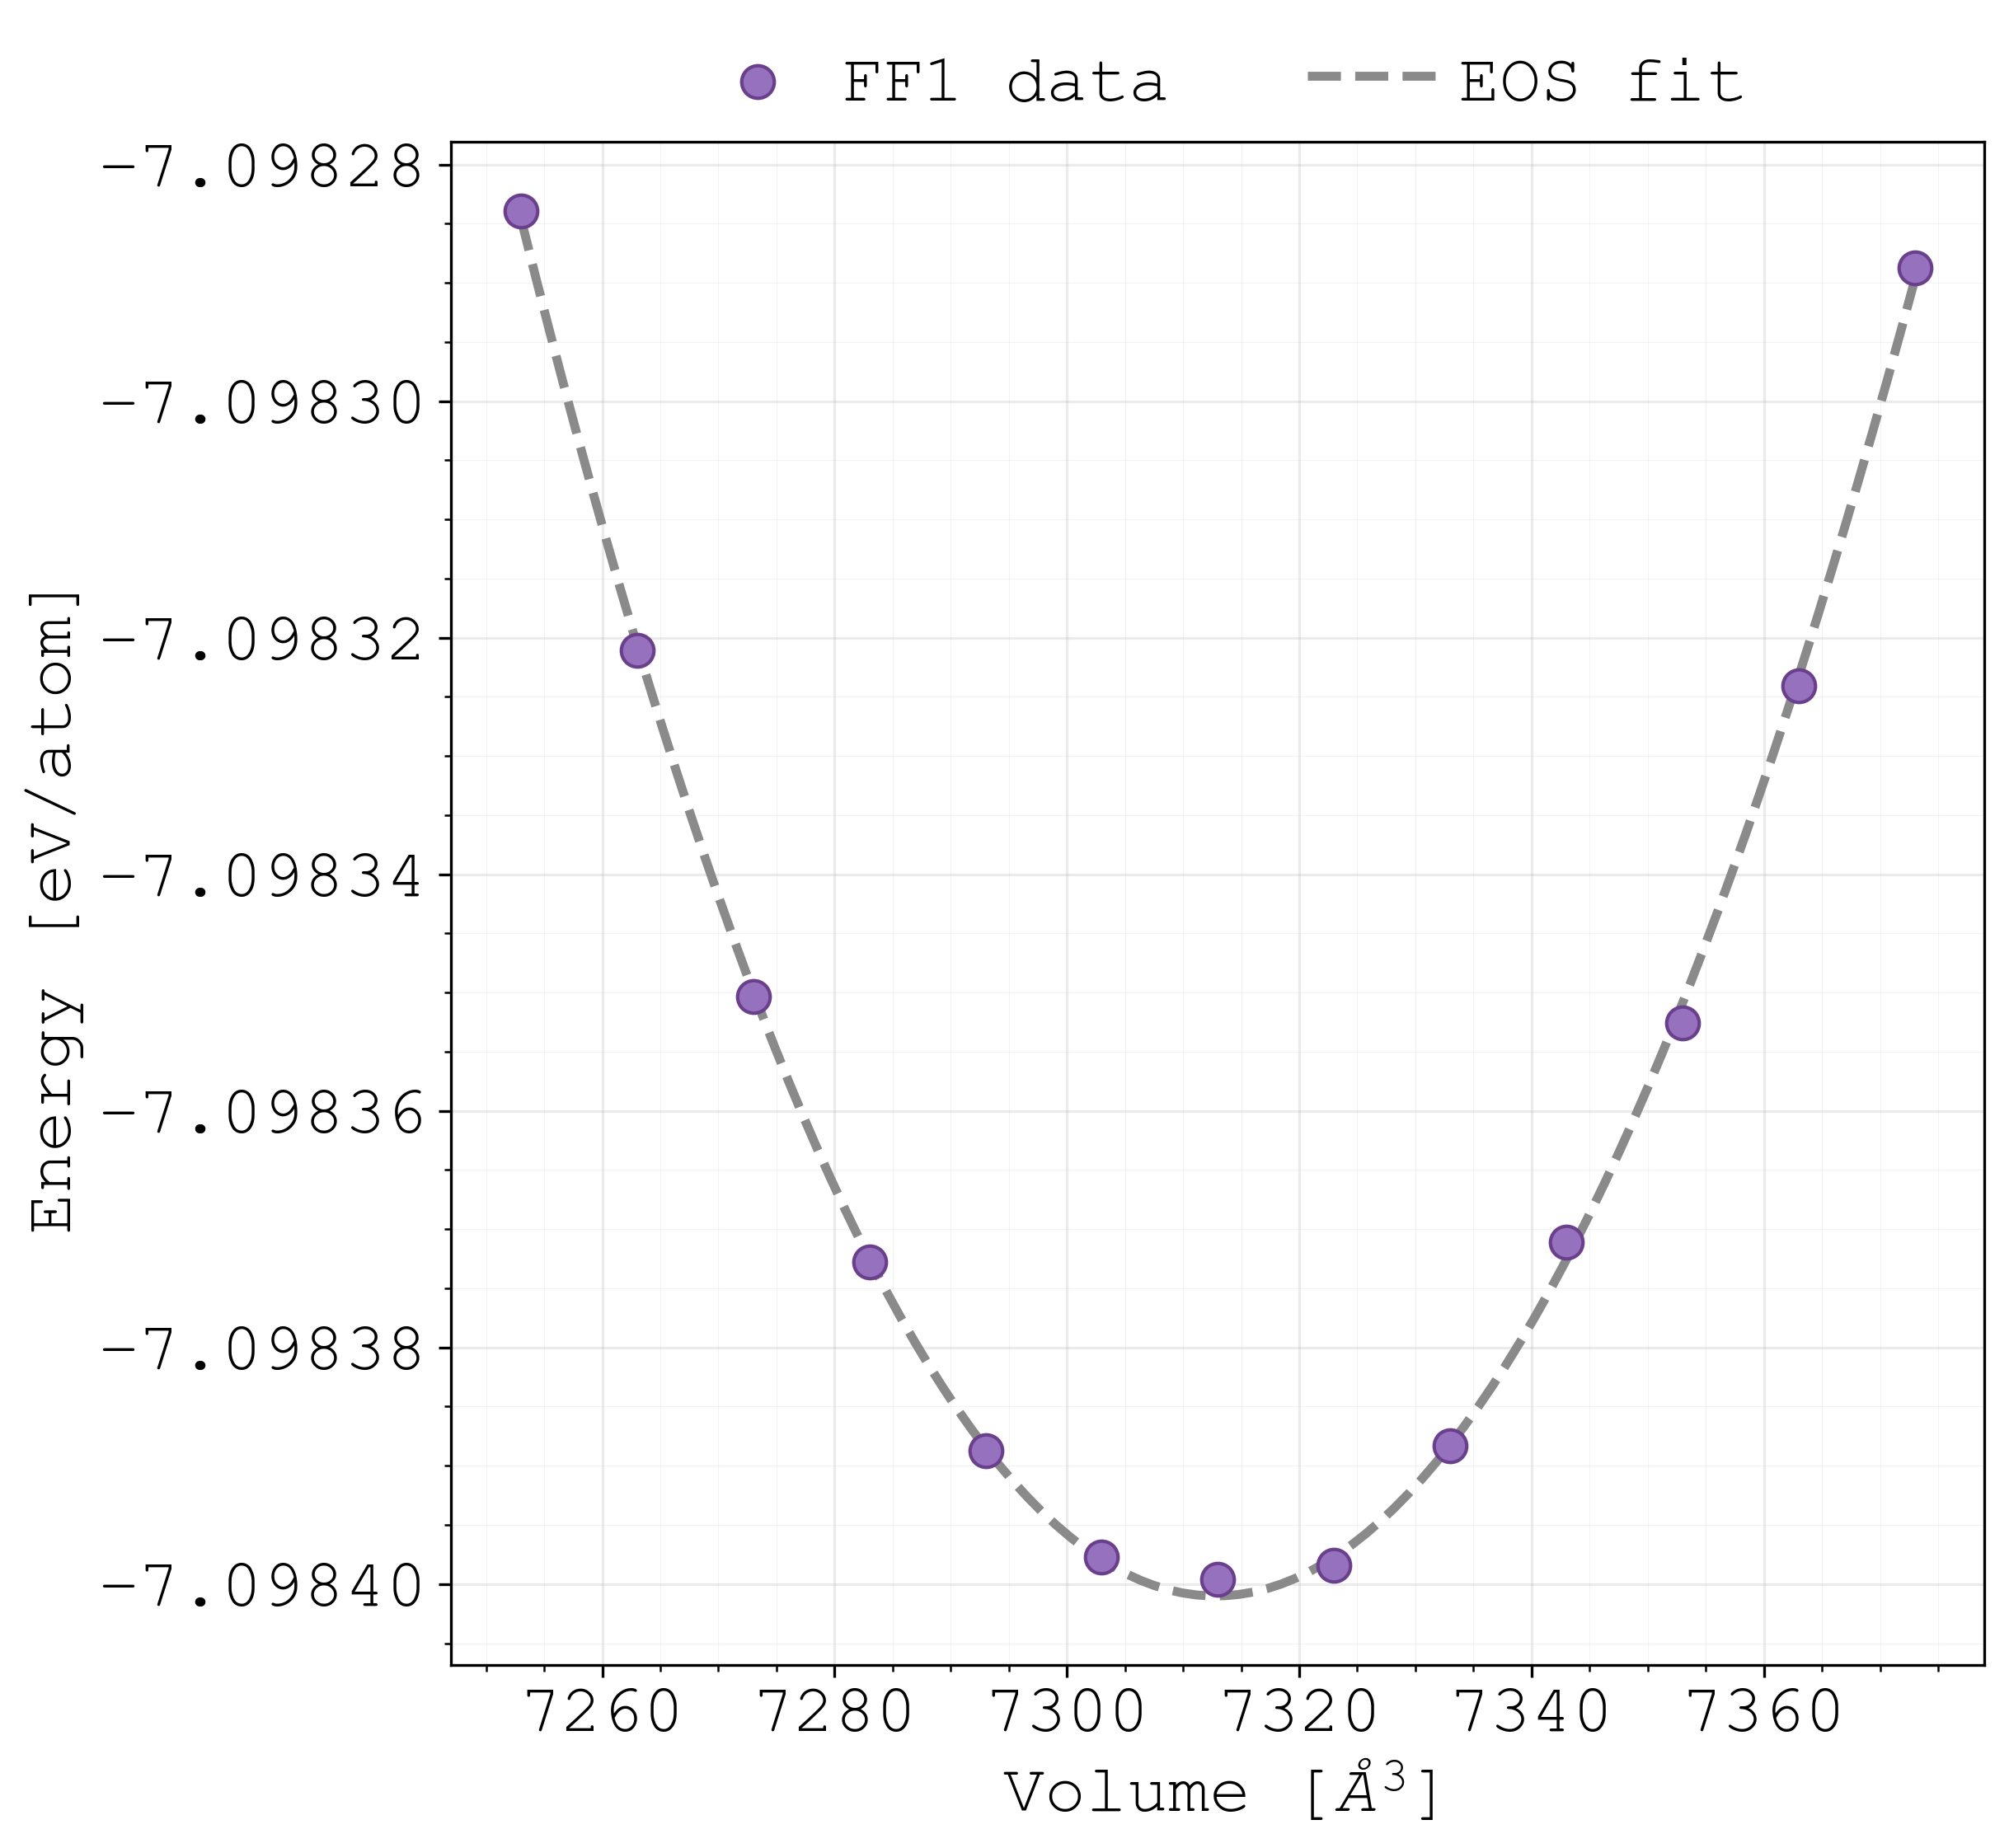
\includegraphics[width=0.7\textwidth]{EOS-FF1.png}
    \caption{Hey}
    \label{fig:eos-ff1}
\end{figure}

\begin{figure}[h]
    \centering
    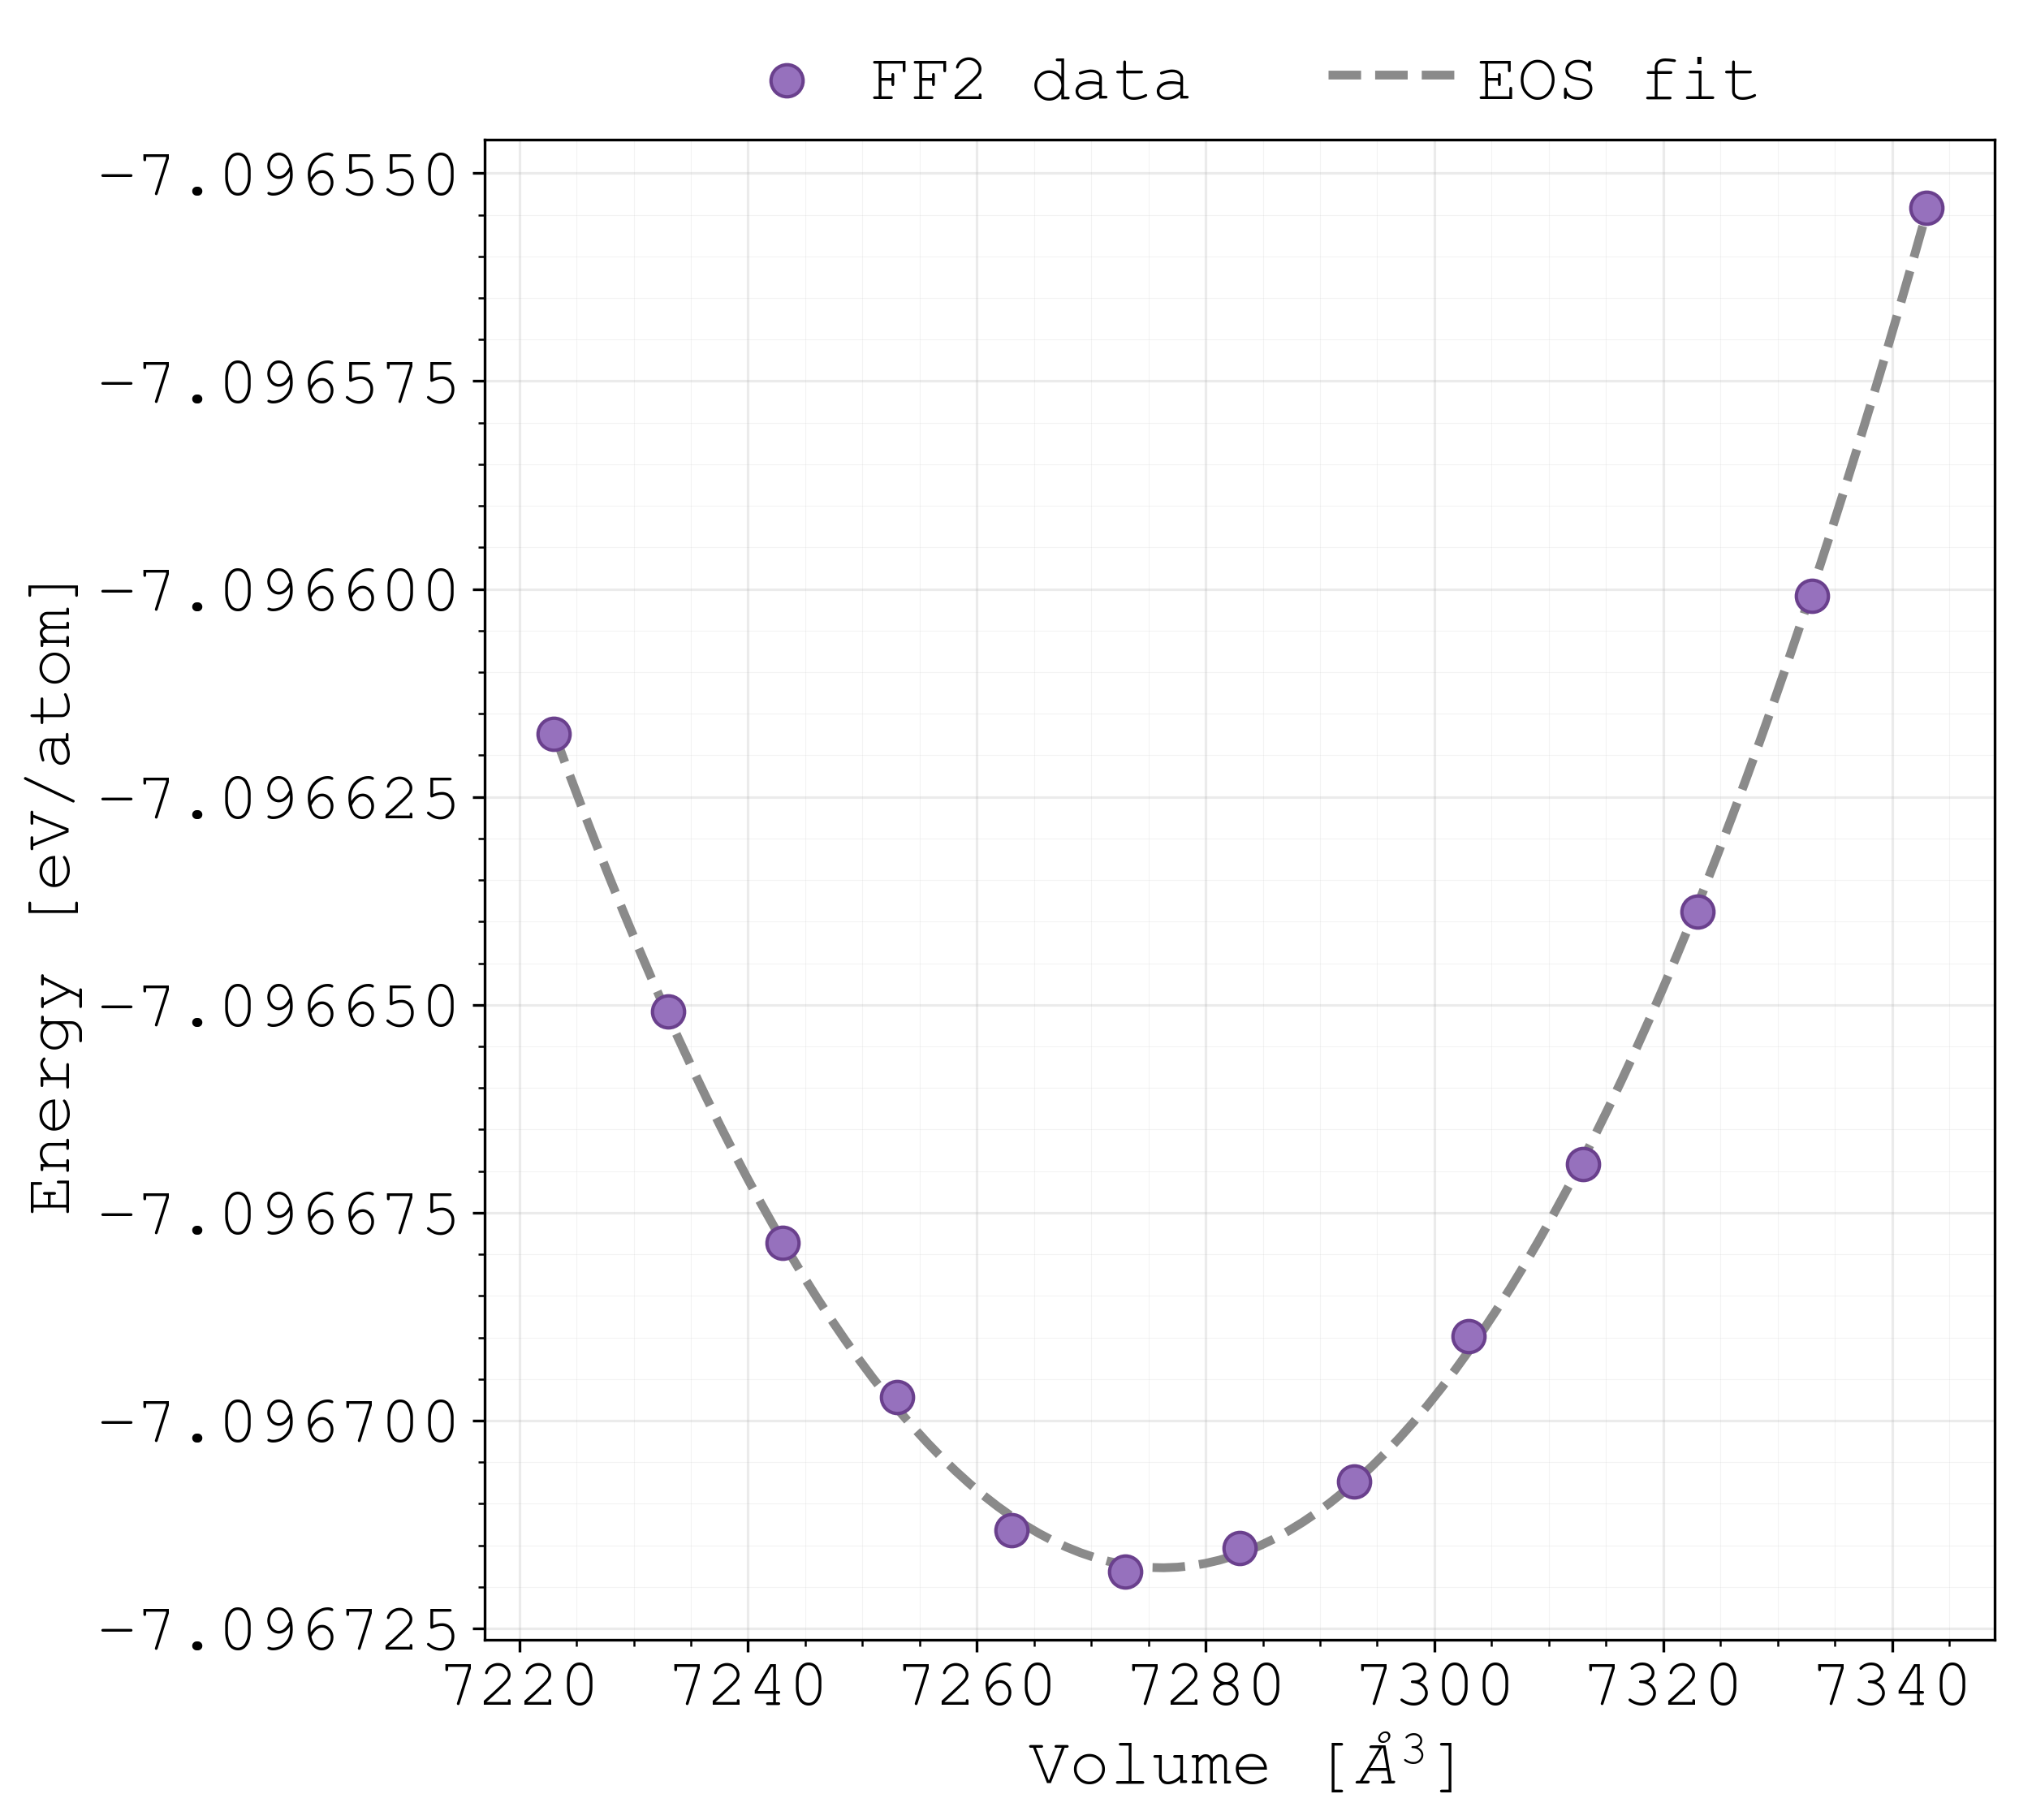
\includegraphics[width=0.7\textwidth]{EOS-FF2.png}
    \caption{Hey}
    \label{fig:eos-ff2}
\end{figure}

\begin{figure}[h]
    \centering
    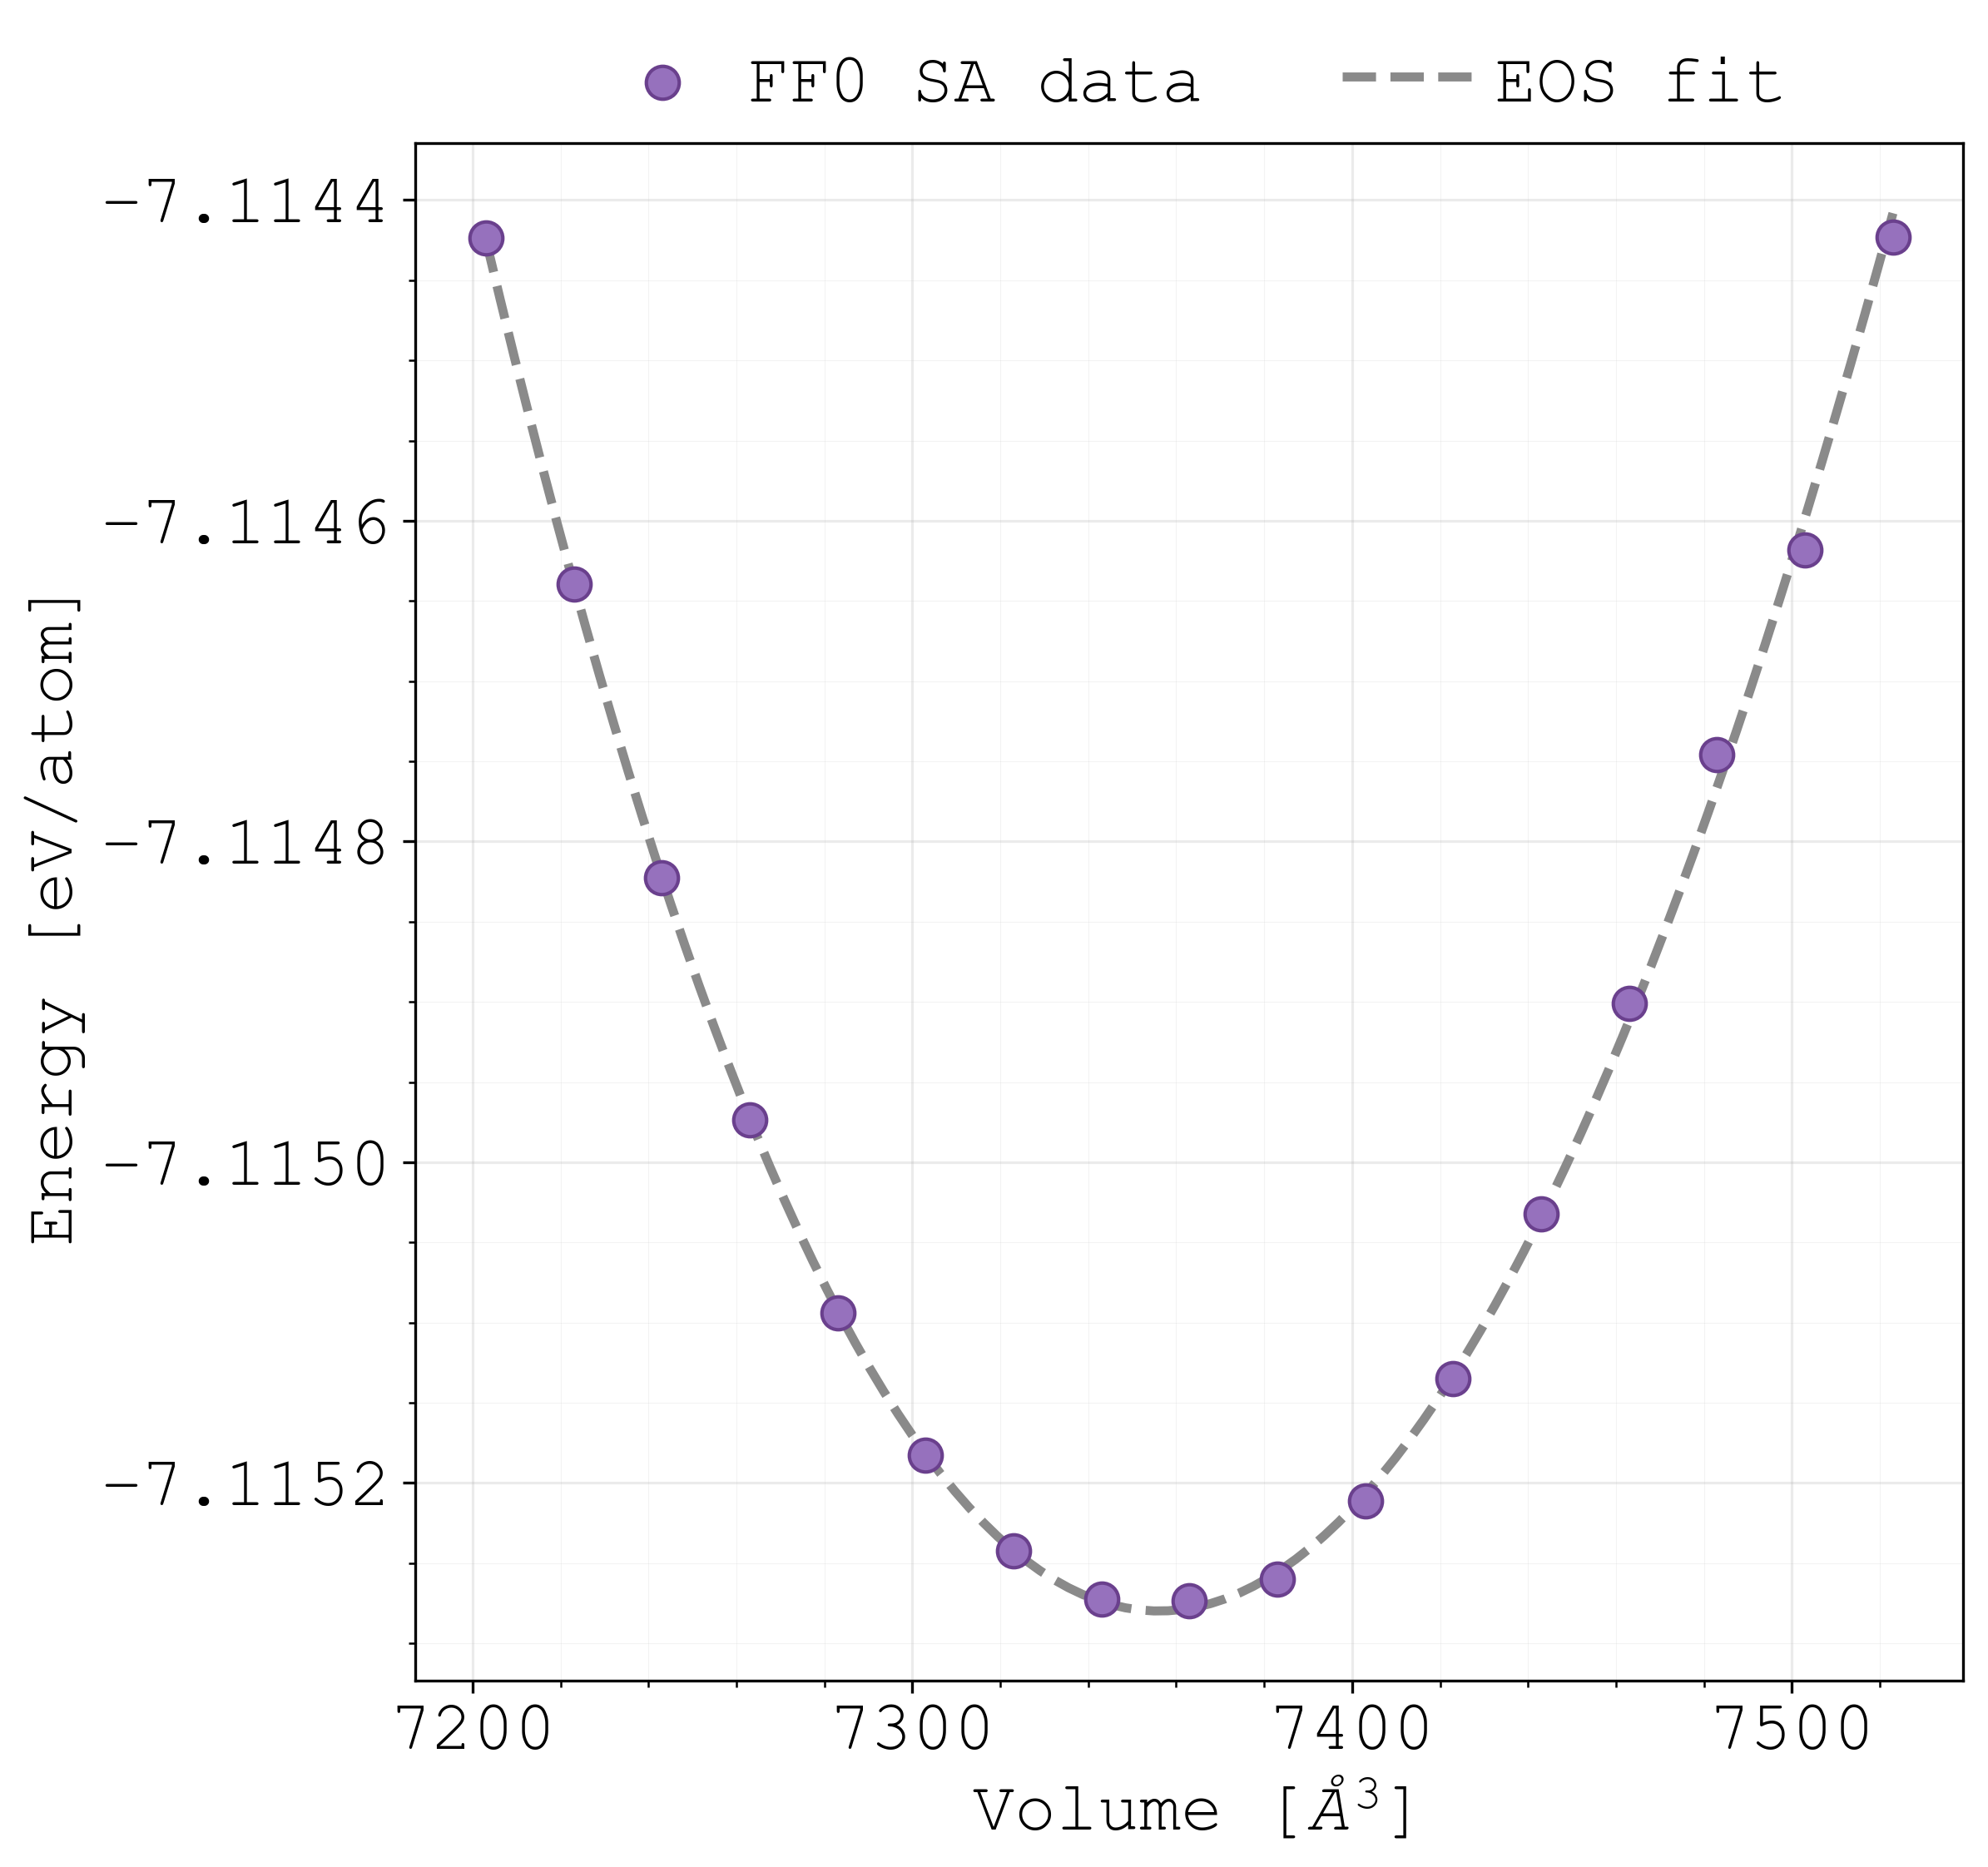
\includegraphics[width=0.7\textwidth]{EOS-SA-FF0.png}
    \caption{Hey}
    \label{fig:eos-sa-ff0}
\end{figure}


\section{Transferability of MLFFs and Thermal Expansion Coefficient of CSH}


\begin{figure}[h]
    \centering
    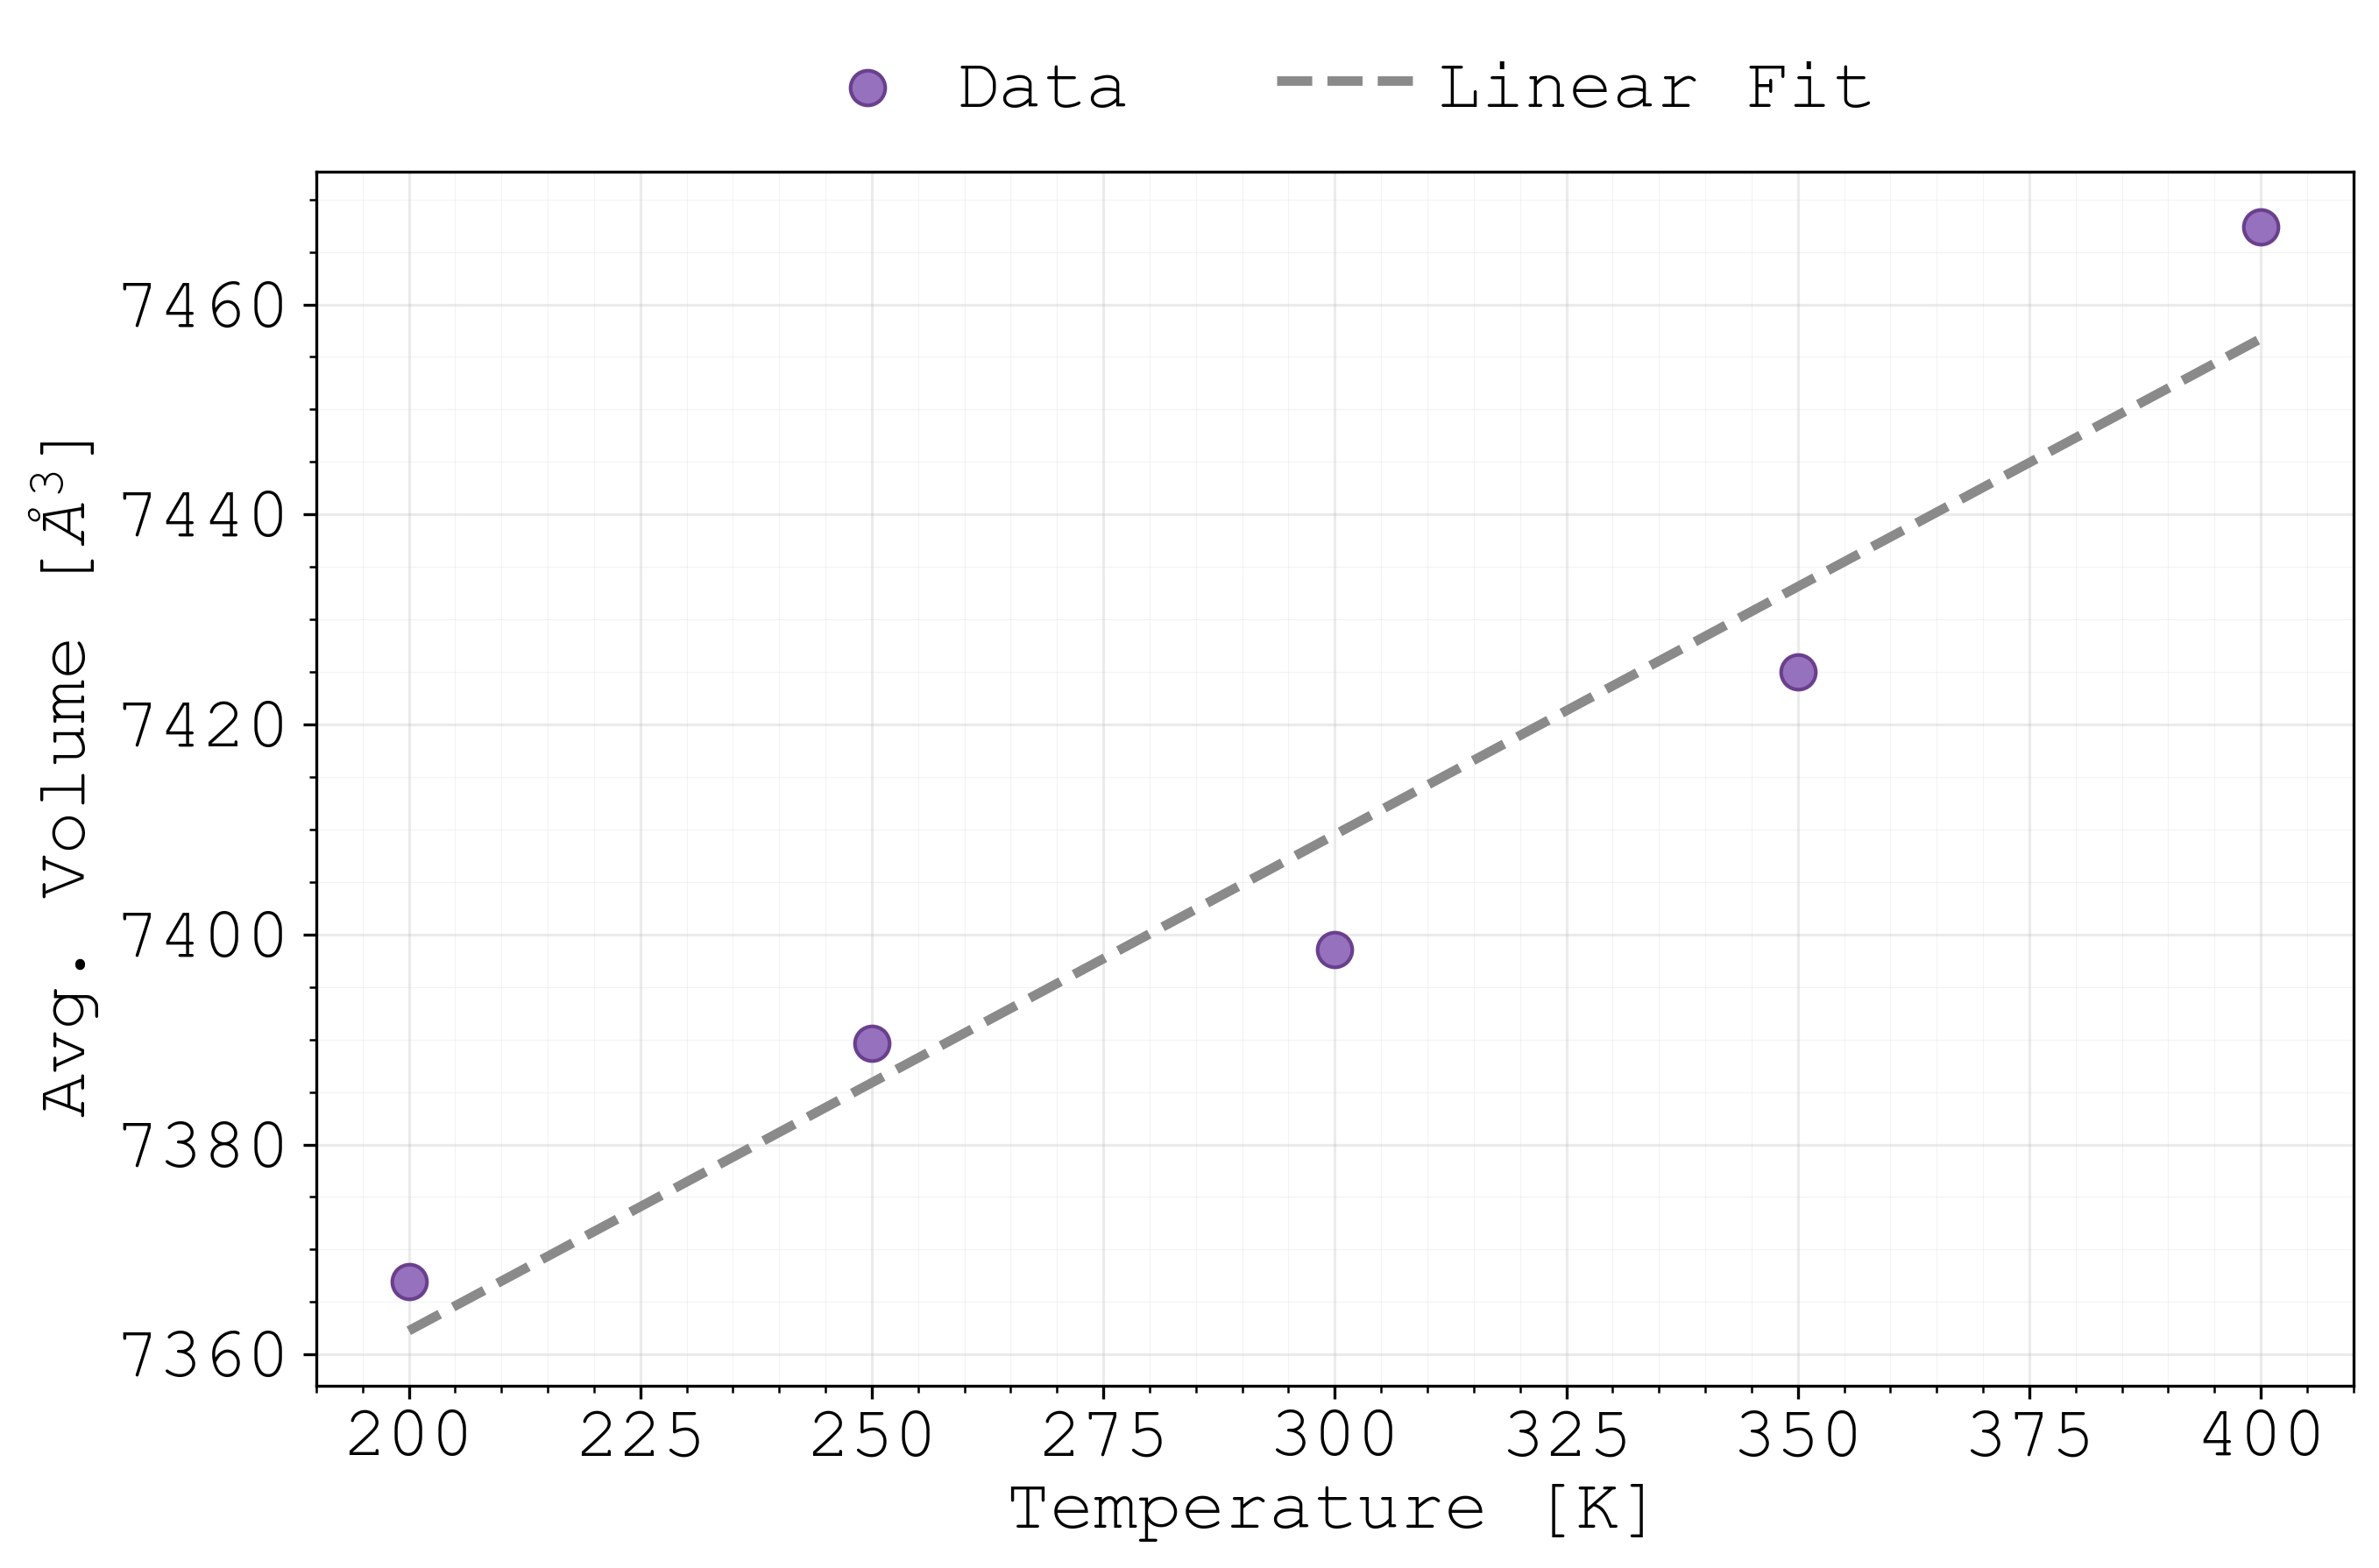
\includegraphics[width=0.8\textwidth]{expansion-coef.png}
    \caption{
    My label
    }
    \label{expansion-coef}
\end{figure}






